% Options for packages loaded elsewhere
\PassOptionsToPackage{unicode}{hyperref}
\PassOptionsToPackage{hyphens}{url}
%
\documentclass[
  man,floatsintext]{apa7}
\usepackage{amsmath,amssymb}
\usepackage{iftex}
\ifPDFTeX
  \usepackage[T1]{fontenc}
  \usepackage[utf8]{inputenc}
  \usepackage{textcomp} % provide euro and other symbols
\else % if luatex or xetex
  \usepackage{unicode-math} % this also loads fontspec
  \defaultfontfeatures{Scale=MatchLowercase}
  \defaultfontfeatures[\rmfamily]{Ligatures=TeX,Scale=1}
\fi
\usepackage{lmodern}
\ifPDFTeX\else
  % xetex/luatex font selection
\fi
% Use upquote if available, for straight quotes in verbatim environments
\IfFileExists{upquote.sty}{\usepackage{upquote}}{}
\IfFileExists{microtype.sty}{% use microtype if available
  \usepackage[]{microtype}
  \UseMicrotypeSet[protrusion]{basicmath} % disable protrusion for tt fonts
}{}
\makeatletter
\@ifundefined{KOMAClassName}{% if non-KOMA class
  \IfFileExists{parskip.sty}{%
    \usepackage{parskip}
  }{% else
    \setlength{\parindent}{0pt}
    \setlength{\parskip}{6pt plus 2pt minus 1pt}}
}{% if KOMA class
  \KOMAoptions{parskip=half}}
\makeatother
\usepackage{xcolor}
\usepackage{graphicx}
\makeatletter
\newsavebox\pandoc@box
\newcommand*\pandocbounded[1]{% scales image to fit in text height/width
  \sbox\pandoc@box{#1}%
  \Gscale@div\@tempa{\textheight}{\dimexpr\ht\pandoc@box+\dp\pandoc@box\relax}%
  \Gscale@div\@tempb{\linewidth}{\wd\pandoc@box}%
  \ifdim\@tempb\p@<\@tempa\p@\let\@tempa\@tempb\fi% select the smaller of both
  \ifdim\@tempa\p@<\p@\scalebox{\@tempa}{\usebox\pandoc@box}%
  \else\usebox{\pandoc@box}%
  \fi%
}
% Set default figure placement to htbp
\def\fps@figure{htbp}
\makeatother
\setlength{\emergencystretch}{3em} % prevent overfull lines
\providecommand{\tightlist}{%
  \setlength{\itemsep}{0pt}\setlength{\parskip}{0pt}}
\setcounter{secnumdepth}{-\maxdimen} % remove section numbering
% Make \paragraph and \subparagraph free-standing
\makeatletter
\ifx\paragraph\undefined\else
  \let\oldparagraph\paragraph
  \renewcommand{\paragraph}{
    \@ifstar
      \xxxParagraphStar
      \xxxParagraphNoStar
  }
  \newcommand{\xxxParagraphStar}[1]{\oldparagraph*{#1}\mbox{}}
  \newcommand{\xxxParagraphNoStar}[1]{\oldparagraph{#1}\mbox{}}
\fi
\ifx\subparagraph\undefined\else
  \let\oldsubparagraph\subparagraph
  \renewcommand{\subparagraph}{
    \@ifstar
      \xxxSubParagraphStar
      \xxxSubParagraphNoStar
  }
  \newcommand{\xxxSubParagraphStar}[1]{\oldsubparagraph*{#1}\mbox{}}
  \newcommand{\xxxSubParagraphNoStar}[1]{\oldsubparagraph{#1}\mbox{}}
\fi
\makeatother
% definitions for citeproc citations
\NewDocumentCommand\citeproctext{}{}
\NewDocumentCommand\citeproc{mm}{%
  \begingroup\def\citeproctext{#2}\cite{#1}\endgroup}
\makeatletter
 % allow citations to break across lines
 \let\@cite@ofmt\@firstofone
 % avoid brackets around text for \cite:
 \def\@biblabel#1{}
 \def\@cite#1#2{{#1\if@tempswa , #2\fi}}
\makeatother
\newlength{\cslhangindent}
\setlength{\cslhangindent}{1.5em}
\newlength{\csllabelwidth}
\setlength{\csllabelwidth}{3em}
\newenvironment{CSLReferences}[2] % #1 hanging-indent, #2 entry-spacing
 {\begin{list}{}{%
  \setlength{\itemindent}{0pt}
  \setlength{\leftmargin}{0pt}
  \setlength{\parsep}{0pt}
  % turn on hanging indent if param 1 is 1
  \ifodd #1
   \setlength{\leftmargin}{\cslhangindent}
   \setlength{\itemindent}{-1\cslhangindent}
  \fi
  % set entry spacing
  \setlength{\itemsep}{#2\baselineskip}}}
 {\end{list}}
\usepackage{calc}
\newcommand{\CSLBlock}[1]{\hfill\break\parbox[t]{\linewidth}{\strut\ignorespaces#1\strut}}
\newcommand{\CSLLeftMargin}[1]{\parbox[t]{\csllabelwidth}{\strut#1\strut}}
\newcommand{\CSLRightInline}[1]{\parbox[t]{\linewidth - \csllabelwidth}{\strut#1\strut}}
\newcommand{\CSLIndent}[1]{\hspace{\cslhangindent}#1}
\ifLuaTeX
\usepackage[bidi=basic]{babel}
\else
\usepackage[bidi=default]{babel}
\fi
\babelprovide[main,import]{english}
% get rid of language-specific shorthands (see #6817):
\let\LanguageShortHands\languageshorthands
\def\languageshorthands#1{}
\ifLuaTeX
  \usepackage[english]{selnolig} % disable illegal ligatures
\fi
% Manuscript styling
\usepackage{upgreek}
\captionsetup{font=singlespacing,justification=justified}

% Table formatting
\usepackage{longtable}
\usepackage{lscape}
% \usepackage[counterclockwise]{rotating}   % Landscape page setup for large tables
\usepackage{multirow}		% Table styling
\usepackage{tabularx}		% Control Column width
\usepackage[flushleft]{threeparttable}	% Allows for three part tables with a specified notes section
\usepackage{threeparttablex}            % Lets threeparttable work with longtable

% Create new environments so endfloat can handle them
% \newenvironment{ltable}
%   {\begin{landscape}\centering\begin{threeparttable}}
%   {\end{threeparttable}\end{landscape}}
\newenvironment{lltable}{\begin{landscape}\centering\begin{ThreePartTable}}{\end{ThreePartTable}\end{landscape}}

% Enables adjusting longtable caption width to table width
% Solution found at http://golatex.de/longtable-mit-caption-so-breit-wie-die-tabelle-t15767.html
\makeatletter
\newcommand\LastLTentrywidth{1em}
\newlength\longtablewidth
\setlength{\longtablewidth}{1in}
\newcommand{\getlongtablewidth}{\begingroup \ifcsname LT@\roman{LT@tables}\endcsname \global\longtablewidth=0pt \renewcommand{\LT@entry}[2]{\global\advance\longtablewidth by ##2\relax\gdef\LastLTentrywidth{##2}}\@nameuse{LT@\roman{LT@tables}} \fi \endgroup}

% \setlength{\parindent}{0.5in}
% \setlength{\parskip}{0pt plus 0pt minus 0pt}

% Overwrite redefinition of paragraph and subparagraph by the default LaTeX template
% See https://github.com/crsh/papaja/issues/292
\makeatletter
\renewcommand{\paragraph}{\@startsection{paragraph}{4}{\parindent}%
  {0\baselineskip \@plus 0.2ex \@minus 0.2ex}%
  {-1em}%
  {\normalfont\normalsize\bfseries\itshape\typesectitle}}

\renewcommand{\subparagraph}[1]{\@startsection{subparagraph}{5}{1em}%
  {0\baselineskip \@plus 0.2ex \@minus 0.2ex}%
  {-\z@\relax}%
  {\normalfont\normalsize\itshape\hspace{\parindent}{#1}\textit{\addperi}}{\relax}}
\makeatother

\makeatletter
\usepackage{etoolbox}
\patchcmd{\maketitle}
  {\section{\normalfont\normalsize\abstractname}}
  {\section*{\normalfont\normalsize\abstractname}}
  {}{\typeout{Failed to patch abstract.}}
\patchcmd{\maketitle}
  {\section{\protect\normalfont{\@title}}}
  {\section*{\protect\normalfont{\@title}}}
  {}{\typeout{Failed to patch title.}}
\makeatother

\usepackage{xpatch}
\makeatletter
\xapptocmd\appendix
  {\xapptocmd\section
    {\addcontentsline{toc}{section}{\appendixname\ifoneappendix\else~\theappendix\fi: #1}}
    {}{\InnerPatchFailed}%
  }
{}{\PatchFailed}
\makeatother
\keywords{big team science, team science, authorship, credit}
\usepackage{lineno}

\linenumbers
\usepackage{csquotes}
\makeatletter
\renewcommand{\paragraph}{@startsection{paragraph}{4}{\parindent}%
  {0\baselineskip @plus 0.2ex @minus 0.2ex}%
  {-1em}%
  {\normalfont\normalsize\bfseries\typesectitle}}

\renewcommand{\subparagraph}[1]{@startsection{subparagraph}{5}{1em}%
  {0\baselineskip @plus 0.2ex @minus 0.2ex}%
  {-\z@\relax}%
  {\normalfont\normalsize\bfseries\itshape\hspace{\parindent}{#1}\textit{\addperi}}{\relax}}
\makeatother

\usepackage{bookmark}
\IfFileExists{xurl.sty}{\usepackage{xurl}}{} % add URL line breaks if available
\urlstyle{same}
\hypersetup{
  pdftitle={What defines big team science?},
  pdfauthor={Erin M. Buchanan1 \& Savannah C. Lewis2},
  pdflang={en-EN},
  pdfkeywords={big team science, team science, authorship, credit},
  hidelinks,
  pdfcreator={LaTeX via pandoc}}

\title{What defines big team science?}
\author{Erin M. Buchanan\textsuperscript{1} \& Savannah C. Lewis\textsuperscript{2}}
\date{}


\shorttitle{Big Team Science}

\authornote{

Erin M. Buchanan is a Professor of Cognitive Analytics at Harrisburg University of Science and Technology. Savannah C. Lewis is a graduate student at the University of Alabama.

Thank you to Dwayne Lieck for providing an extensive list of large scale projects for this manuscript.

Preprint: \url{https://osf.io/hqta4/}

The authors made the following contributions. Erin M. Buchanan: Conceptualization, Data curation, Formal Analysis, Methodology, Project administration, Visualization, Writing -- original draft, Writing -- review \& editing; Savannah C. Lewis: Conceptualization, Data curation, Methodology, Project administration, Writing -- original draft, Writing -- review \& editing.

Correspondence concerning this article should be addressed to Erin M. Buchanan, 326 Market St., Harrisburg, PA 17101. E-mail: \href{mailto:ebuchanan@harrisburgu.edu}{\nolinkurl{ebuchanan@harrisburgu.edu}}

}

\affiliation{\vspace{0.5cm}\textsuperscript{1} Harrisburg University of Science and Technology\\\textsuperscript{2} University of Alabama}

\abstract{%
This study presents the first large-scale, data-driven analysis of authorship in Big Team Science (BTS) drawing on over half a million articles across four scientific domains. Using the top decile of the data, we defined BTS as collaborations with 11+ authors across six or more institutions. We compared BTS with traditional team science to investigate changes in publication rates, authorship characteristics, and global representation. Publication rates for traditional team science and BTS have both risen over time, but the growth trajectory varies depending on the subject area. We found that early-career researchers are increasingly represented in both BTS and smaller teams, suggesting greater accessibility over time. Leadership roles remain concentrated in high-income, WEIRD regions for smaller teams. This work contributes a replicable, empirical definition of BTS and highlights the need for more equitable recognition and inclusion in large-scale scientific collaboration.

\section{General Disclosures}\label{general-disclosures}

Conflicts of interest: Both authors declare no conflicts of interest.

Funding: No funding was obtained for this project.

Artificial Intelligence: Artificial Intelligence tools (e.g., ChatGPT) were used to assist in debugging and resolving coding errors.

Ethics: No ethics review was necessary for this project.

Computational reproducibility: A reproducible version of this manuscript can be found at: \url{https://doi.org/10.24433/CO.2018846.v1}, which is linked to GitHub (\url{https://github.com/doomlab/big_team_who}) and archived at Zenodo (\url{https://doi.org/10.5281/zenodo.15936025}). Elsevier has authorized use of the Scopus database to execute and validate the code for retrieving and summarizing article records. Although we cannot distribute Scopus data directly, we provide all code, processing steps, and derived outputs necessary to reproduce the analyses presented in this manuscript.

Pre-registration: This manuscript was preregistered with the same conceptual ideas using Google Scholar and ORC-ID databases (\url{https://doi.org/10.17605/OSF.IO/F2DTR}) but then was updated with access to the Scopus database for a broader picture of BTS projects (\url{https://doi.org/10.17605/OSF.IO/FHEUN}). After peer review, the pre-registration was updated to address the unclear definition of big team science to focus on a data-driven definition to explore the research questions.

Materials: All study materials are publicly available (\url{https://doi.org/10.5281/zenodo.15936025}).

Data: All data from Scopus outputs are publicly available (\url{https://doi.org/10.5281/zenodo.15936025}).

Analysis scripts: All analysis scripts are publicly available (\url{https://doi.org/10.5281/zenodo.15936025}).
}



\begin{document}
\maketitle

Scientific discovery has increasingly become a collaborative process,
with the scale and scope of team science have dramatically expanded in
recent years (Council et al., 2015). Collaboration in scientific endeavors
involves multiple researchers (potentiality) at multiple institutions to
communicate and work together to advance knowledge in their chosen
field(s). This unique composition of a collaboration for each project is
dependent on the skill sets, hypotheses, and perspectives of collaborators
involved. A key strength of collaboration lies in its flexibility, allowing it
to adapt to the needs of the project and the researchers themselves. While collaboration is not new in science, interest in ``team science'' is
growing as individual researchers seek an interdisciplinary approach to
research or bring on more students to their project. Team science is
often defined as groups of researchers with various expertise working
together to investigate complex problems (Fiore, 2008). Unlike general
collaboration, team science involves structured roles, coordinated
workflows, and shared resources to address challenges that would be
difficult for individual researchers or one small team to solve
independently.

The movement toward team science reflects demands of modern research to
answer complex questions, meet funding agencies and universities desires for
interdisciplinary research, and the desire to increase scientific representation
(Council et al., 2015). Further, the evolution of team science reflects broader shifts
in research practices, driven by two sources: 1) increasing globalization
and technology that allows for real-time interdisciplinary research (B. F. Jones et al., 2008), and 2) expanding interest in reproducibility, replication,
and generalizability (i.e., the credibility movement, Maxwell et al., 2015; Nelson et al., 2018; Vazire et al., 2022; Zwaan et al., 2018). Technological advances have provided easier ways to
collaborate with people who are from other universities and countries
through document sharing platforms (e.g., Google, GitHub, and the Open
Science Framework), video chatting platforms (e.g., Zoom, Microsoft
Teams), and messaging and project management platforms (e.g., Slack,
Trello, when2meet, etc.).

The credibility movement has been the main catalyst for the increased
interest and broader shift of research practices. The movement
emphasizes reproducibility and transparency in science, encouraging
researchers to form new ways to increase the rigor in scientific
endeavors. Throughout the last decade, the credibility movement has
pushed for larger, more diverse teams and the involvement of
participants from varied backgrounds. This shift in teams and
participants focuses on increasing credibility, generalizability, and
reliability of scientific findings. This form of collaboration has been
coined ``Big Team Science.'' Big Team Science (BTS) builds on team science
by scaling efforts to include larger, often globally diverse teams,
which requires significant coordination and infrastructure (Coles et al., 2022; Forscher et al., 2022; N. Stewart et al., 2017). BTS projects and organizations organize
extensive collaborations, intentionally incorporating diverse
populations and perspectives into research. This large-scale approach
enhances the reliability and generalizability of findings by integrating
varied methodologies and viewpoints, leading to more robust and
inclusive scientific outcomes. BTS organizations often pool extensive
networks of researchers and resources, aiming to tackle grand scientific
challenges that would be difficult to address within smaller or less
coordinated collaborations. By having both collaborations that span
across the globe and subfields of research areas, age groups, and
education levels should help to drive science in the path of better
materials, reliability, generalizability, and more robust sample sizes
in a study (Auspurg \& Brüderl, 2021; LeBel et al., 2018; Nosek \& Lakens, 2014a).

For example, psychology has seen an increase in BTS publications like
the Open Science Collaboration (Open Science Collaboration, 2015), Many
Labs Collaborations (Buttrick et al., 2020; Ebersole et al., 2016, 2020; Klein et al., 2018; Klein et al., 2022; Mathur et al., 2020; Skorb et al., 2020) or the first papers
from the Psychological Science Accelerator (Bago et al., 2022; Buchanan et al., 2023; Dorison et al., 2022; B. C. Jones et al., 2021; Moshontz et al., 2018; Psychological Science Accelerator Self-Determination Theory Collaboration, 2022; Wang et al., 2021). The success and interest in the large-scale
reproducibility projects (Errington et al., 2021; Open Science Collaboration, 2015), paired with the meta-scientific publications
focusing on researcher practices and incentive structures
(John et al., 2012; Silberzahn et al., 2018) led to a change in journal guidelines
and incentives for researchers interested in participating in
large-scale studies overall (Grahe, 2014; Kidwell et al., 2016; Mayo-Wilson et al., 2021; Nosek et al., 2015). In some fields, the BTS movement demonstrated that
large-scale teams were a practical (and publishable) solution to
answering research questions in generalizable way. The support for
Registered Reports, papers accepted before the data has been collected
(Nosek \& Lakens, 2014b; S. Stewart et al., 2020), has allowed researchers to invest in
projects that they know should be published when the project is
complete. Further, the implementation of the Transparency and Openness
Guidelines (Nosek et al., 2015) and the Contributor Role Taxonomy (CRediT)
system (Allen et al., 2019) have pushed journals and researchers to promote more
open, inclusive publication practices.

Beyond replication concerns, the credibility movement has mirrored calls
for diversification or de-WEIRDing (e.g., Western, Educated,
Industrialized, Rich, and Democratic) scientific research (Henrich et al., 2010; Newson et al., 2021; Rad et al., 2018) by improving representation in research samples.
Like the large-scale studies in Physics ({``A Philosophical Case for Big Physics,''} 2021; Castelnovo et al., 2018)
and Biology (Collins et al., 2003), the Social Sciences struggle to represent
the breadth of humanity across both researcher and population
characteristics. Now, grassroots organizations, such as the
Psychological Science Accelerator (\url{https://psysciacc.org}), ManyBabies
(\url{https://manybabies.github.io/}), NutNet (\url{https://nutnet.org/}),
DRAGNet (\url{https://dragnetglobal.weebly.com/}), and IceCube
(\url{https://icecube.wisc.edu/}) can begin to tackle these issues by
recruiting research labs from all over the globe to provide diversity in
geographic, linguistic, and researcher representation. Publications have
examined the global understanding of morality, face processing, COVID-19
information signaling, and more (Bago et al., 2022; Dorison et al., 2022; B. C. Jones et al., 2021; Psychological Science Accelerator Self-Determination Theory Collaboration, 2022; Van Bavel et al., 2022; Wang et al., 2021). While these organizations and one-time groups
for BTS studies have provided an incredible wealth of data for the
scientific community, we do not yet know exactly how to define BTS: which is generally termed ``an unusually large number of collaborators''
(Coles et al., 2022; Forscher et al., 2022).

The lack of formal definition raises questions about whether it
represents a distinct phenomenon or simply a natural extension of team
science. These big teams pose unique challenges, including coordinating
work across diverse time zones, managing conflicts in decision-making,
and ensuring fair distribution of credit for contributions
(Cummings \& Kiesler, 2007; Wuchty et al., 2007), but also could provide big rewards by
pooling expertise and increased interdisciplinary funding (Fiore, 2008).
This paper seeks to clarify the concept of BTS by first establishing a
data-driven definition based on publication patterns. With this
quantitative distinction in place, we analyze publication trends over
time to assess the trajectories of both traditional team science and
BTS. Furthermore, we investigate the diversity of authors involved in
these collaborations to explore whether shifts in the scientific
landscape, such as efforts to de-WEIRD science and the expansion of
collaborative opportunities, have influenced who participates in team
science and BTS. By synthesizing insights from the growth and
diversification of team science, this paper seeks to critically examine
the emergence of big teams. Specifically, it aims to explore whether big
teams are quantitatively different from traditional collaboration models
with the following research questions.

\section{Research Questions}\label{research-questions}

\begin{itemize}
\tightlist
\item
  Research Question 1: Exploring historical and current publication
  values, what should define big team science versus traditional team science?

  \begin{itemize}
  \tightlist
  \item
    Question 1A: What number of authors and institutional
    affiliations should designate the differences between traditional team science and big team science?
  \item
    Question 1B: Using the definition from 1A, are there changes in
    the number of publications over time?
  \end{itemize}
\item
  Research Question 2: How has the diversity of those involved in traditional team
  science and big team science changed over time?
\end{itemize}

\section{Method}\label{method}

\subsection{Publications}\label{publications}

We used data from 1970-2024 in the Scopus database, as it is noted
online that 1970 and forward includes cited references for calculation
of several of our variables described below. We analyzed our results
based on four subject areas present in the Scopus database: Physical
Sciences, Health Sciences, Social Sciences, and Life Sciences. We used
the subject area split to ensure one field did not dominate BTS
definitions and determine differences in trends across sub-areas of
science. We filtered the database to include articles, articles in
press, business articles, conference papers, data papers, preprints, and
surveys using Elsevier's classification system. This project was
supported by access to the Scopus database through the International
Center for the Study of Research.

\subsection{Data Curation}\label{data-curation}

\subsubsection{RQ1: Defining BTS}\label{rq1-defining-bts}

For each of the publications in Scopus, we calculated the number of
distinct authors and institutions. If an author had multiple
affiliations, we used the first affiliation listed. Each publication was
classified into the four subject areas based on the All Journal Subject
Codes present in the database. Publications can be included in multiple
subject codes. For example, a medical paper may be listed in both life
sciences and health sciences.

\subsubsection{RQ2: Seniority}\label{rq2-seniority}

Career length for each author was defined as the year of the first
publication minus the current year listed for each author. Number of
publications included the number of unique entries an author was
included in the database. Career length and number of publications was
used as a proxy for the ``age'' or ``seniority'' of a scholar.

\subsubsection{RQ2: Geopolitical Region}\label{rq2-geopolitical-region}

Geopolitical region was created by binning country code identifiers into
the 17 identified United Nation subregions.

\section{Results}\label{results}

We used the 95\% confidence interval to make decisions on predictor or
effect size differences from zero. The confidence interval that does not
include zero would be considered different from zero (to four decimal
places). We made no directional predictions.

\subsection{RQ1A: Defining BTS}\label{rq1a-defining-bts}

The total number of papers included in the Scopus database at the time
of this analysis was 97,532,104. 62,966,549
articles were included past 1970 in the defined article types, which
included 53,622,443 distinct authors. We then
filtered the data to include only teams, which was defined as two
authors from at least two institutions. The total number of papers for
team projects was 32,454,393 and
28,353,445 distinct authors. The data was then
classified into subject areas by paper, which lead to missing data. The
final number of papers included was 32,448,373 with
28,350,468 distinct authors. The dataset was
curated to include one row per author, paper, and subject area (i.e.,
long format (Wickham, 2007)) which included
241,269,297 total rows of data.

\begin{figure}
\centering
\pandocbounded{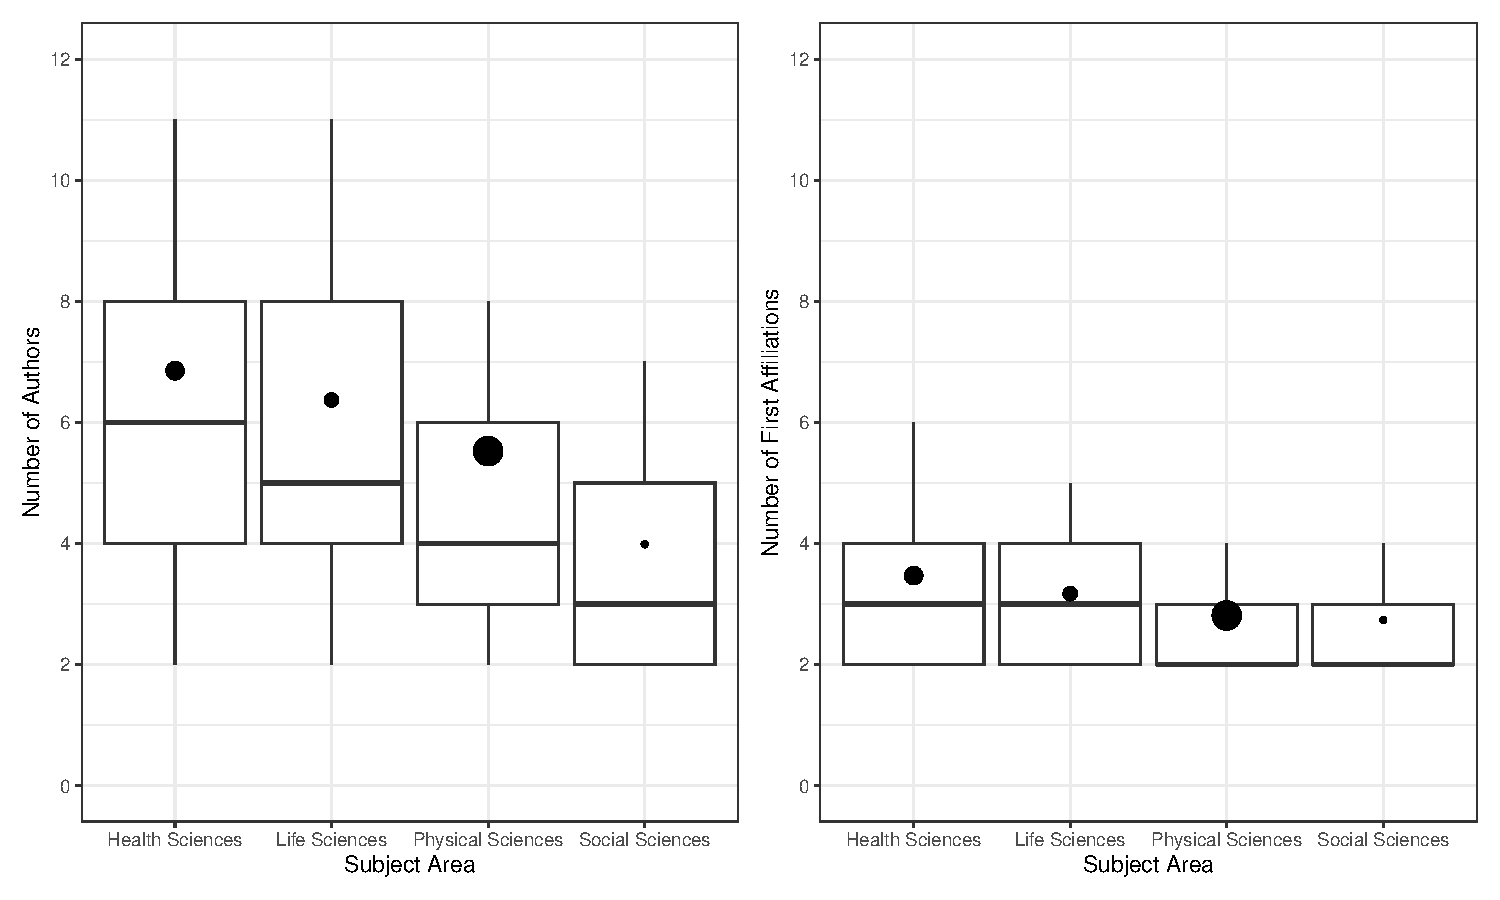
\includegraphics[keepaspectratio]{manuscript_definition_files/figure-latex/fig-stats-authors-1.pdf}}
\caption{\label{fig:fig-stats-authors}The left panel depicts the number of authors included on a paper by subject area, and the right panel demonstrates the number of affiliations by subject area. The boxplot shows the median (bold line), the interquartile range (the box), and the minimum to the 90th percentile of the number of authors/affiliations as the range line. Normally these plots include the entire range of the data, but these extreme range made the boxplot information unreadable. The dots indicate the average number of authors/affiliations for each area with the size of the dot indicating the standard deviation of the statistic. Therefore, larger dots indicate more variability in the number of authors and affiliations.}
\end{figure}

Figure \ref{fig:fig-stats-authors} displays the number of authors and
affiliations by subject area. The figure demonstrates that the median
number of authors is largest for health sciences, followed by life
science, physical sciences, and then social sciences. The general
pattern of team authorship includes about 2-8 authors, from about 2-4
institutions. We used the maximum value (i.e., across all subject areas)
for the 90th percentile as our exploratory definition for big team
papers after examining the results from this analysis. We selected this
percentile to have the high of the distribution, but also to be able to
include enough papers for analysis across time. Therefore, big teams
were defined as 11 authors from at least 6 different institutions.\footnote{In a previous version of this manuscript, we defined big teams as
  10 authors from at least 10 institutions based on our own
  experiences working within a research consortium. All definitions
  are likely subjective, but the definition in this manuscript
  represents the top 10\% of author and affiliations in a large body of
  papers.}

We applied a consistent definition of Big Team Science (BTS) across all four research domains in our analysis. As shown in Figure \ref{fig:fig-stats-authors}, the 90th percentile of team size is consistent across subject areas, varying by only four authors (e.g., from 7 to 11), which supports the use of a unified threshold. Over time (Figure \ref{fig:fig-paper-time}), we observe increasing publication counts in all fields. While social sciences currently lag behind in both volume and growth rate, we anticipate continued growth as more infrastructure and funding are directed toward collaborative efforts in this area. Unlike fields such as health sciences, which often benefit from greater financial resources and institutional support (e.g., through IRBs and clinical networks), social science collaborations face unique structural barriers that may slow their expansion. Additionally, defining BTS consistently across fields is methodologically important because many publications are interdisciplinary and assigned to multiple subject categories. A unified operationalization allows for clearer comparisons and avoids arbitrary distinctions between overlapping research areas.

Supplemental Table \ref{tab:big-teams-table} includes the number of
distinct authors and papers for each subject area by overall teams and
big teams using our 90th percentile definition. The total number of
distinct authors for big team papers was 968,765 with
4,541,369 distinct authors. In RQ2, we split the big team
data into bins using 11-49 authors, 50-99 authors, and 100+ authors groupings for convenience to display/analyze geopolitical regions. The
table shows the number of authors and papers for those analyses.

\subsection{RQ1B: Changes over Time}\label{rq1b-changes-over-time}

For analyzing changes across time, we split the data into traditional team science
projects (2-10 authors, 2-5 affiliations) and BTS projects (as defined
above, 11+ authors, 6+ affiliations). The number of papers found in
Scopus across time for each subject area are displayed in Figure
\ref{fig:fig-paper-time}. The visual results indicated that the number
of traditional team science papers was increasing the most in physical sciences for
all manuscripts, followed by life and health sciences, and the last is
social sciences. Examining only BTS projects shows that the rate is also
increasing across time. All teams appear to start increasing in the
1990s, while BTS projects do not start increasing off floor effects
until past 2000. The health and life sciences show the largest increases
across time in big teams with the smallest trend in the social sciences.

\begin{figure}
\centering
\pandocbounded{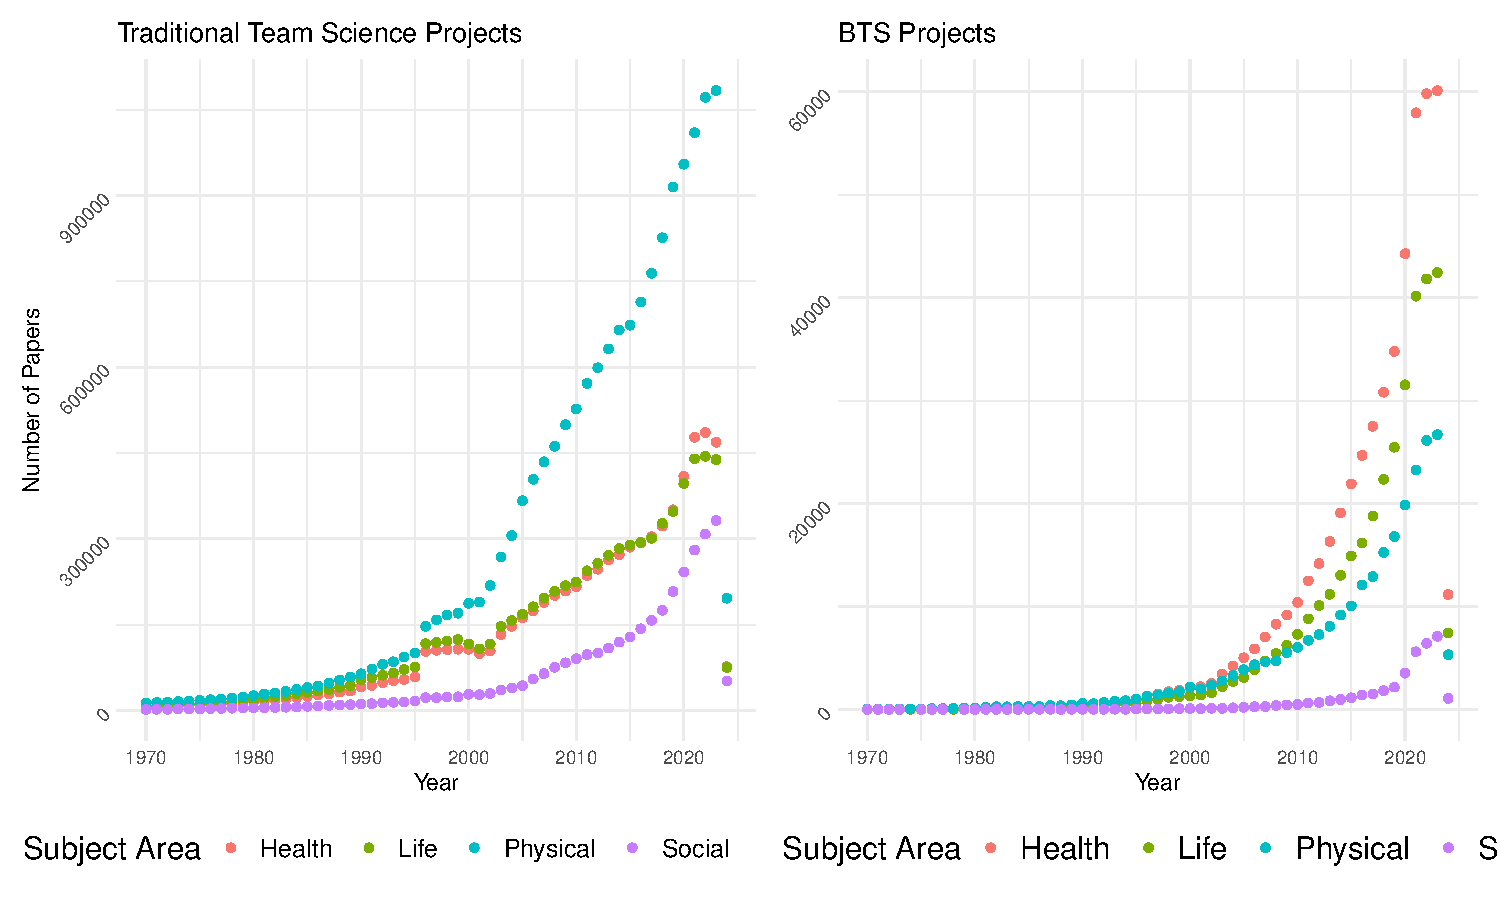
\includegraphics[keepaspectratio]{manuscript_definition_files/figure-latex/fig-paper-time-1.pdf}}
\caption{\label{fig:fig-paper-time}The number of manuscripts across time for all traditional team science papers (left) and big team science papers (right).}
\end{figure}

Using the \texttt{minpack.lm} library (Elzhov et al., 2023), we calculated the
exponential rate of growth for traditional team science and BTS projects, and these
results are shown in Supplemental Figure \ref{fig:rate-estimates-fig}. All growth rate
confidence intervals excluded zero, indicating an exponential increase
in the number of team papers over time. BTS growth rates were always
higher than their traditional team science counterparts, but the 95\% confidence
intervals for the growth estimate overlapped for all statistics.
Therefore, the growth trends, while visually appearing to be different,
were likely similar for each subject area and team size when examined by
estimating exponential growth statistics.

\subsection{RQ2: Seniority}\label{rq2-seniority-1}

\begin{figure}
\centering
\pandocbounded{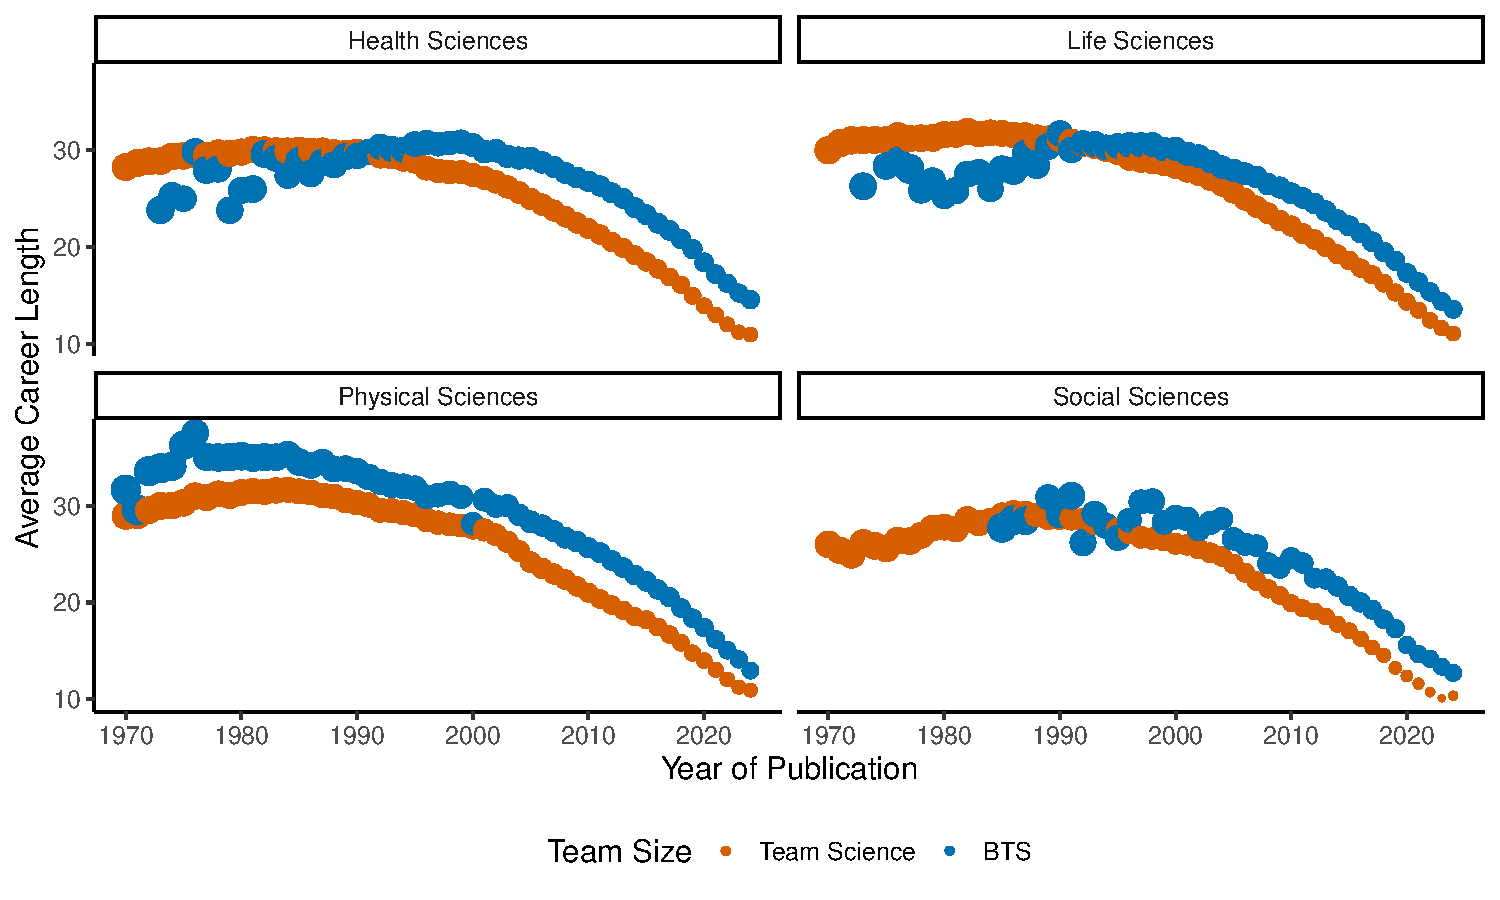
\includegraphics[keepaspectratio]{manuscript_definition_files/figure-latex/fig-career-1.pdf}}
\caption{\label{fig:fig-career}Average career length for big-team science authors. Larger dots indicate more variability in career length for authors by averaging the standard deviation in career length for each manuscript within a year. The data has been filtered to at least 10 publications in a year for this graph.}
\end{figure}

Figure \ref{fig:fig-career} portrays the average career length for
authors involved in traditional team science and BTS projects over time. Career
length was defined as the year of first publication minus the current
year, and higher numbers mean longer careers. The general pattern for
traditional team science and BTS projects is a decrease in average career length
over time. However, it appears that, in at least the last two decades,
BTS projects average a longer career length than traditional team science projects.
This trend is visually consistent across all four subject areas
examined.

\subsubsection{Career Length}\label{career-length}

To analyze these trends over time, we calculated the average career
length for each publication (i.e., averaging author career lengths to
create one score for each paper) and analyzed a regression analysis
using career length to predict year of publication. In order to show
variance between individuals, we calculated the standard deviation of
career length for each publication and used this variance as an
additional predictor. Negative career length slopes would indicate more
young scholars in later years (i.e., lower average career length as time
increases). Positive career length slopes would indicate older scholars
in later years (i.e., higher average career length as time increases).
Negative career variance slopes imply that variability decreases over
the years, so the average career length is more homogeneous. Positive
career length slopes imply that variability increases over the years, so
the average career length is varied across individuals (i.e., different
stages of scholars). Figure \ref{fig:fig-heatmap} displays the results
for all regression analyses.

\begin{figure}
\centering
\pandocbounded{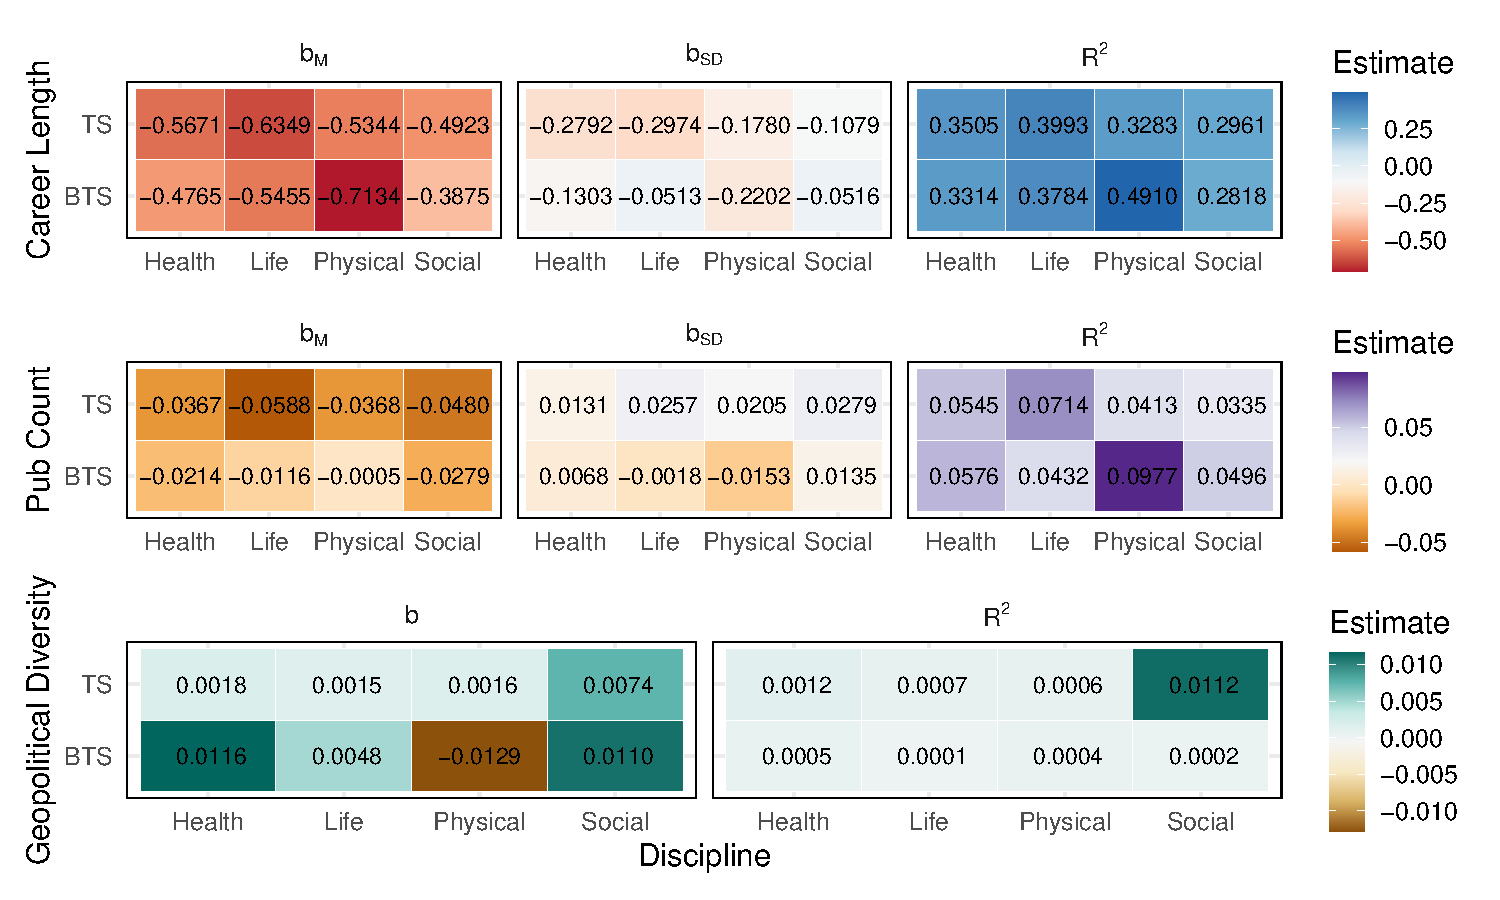
\includegraphics[keepaspectratio]{manuscript_definition_files/figure-latex/fig-heatmap-1.pdf}}
\caption{\label{fig:fig-heatmap}Heatmap results of regression analyses for career length, number of publications, and geopoliticalwithin the region. Each square represents a \emph{b} value or the slope of the predictor (x-axis) onto the dependent variable (each panel), with the exception of the bottom row which is the effect size of each regression analysis \(R^2\). Slopes included both the overall value of the predictor (\(b\), \(b_M\)) and the standard deviation of the predictor over time (\(b_{SD}\)). The color of the square represents the strength of the predictor. The top figure represents all results together for comparison across analyses. The bottom row represents individual heatmaps for each hypothesis to distinguish small differences between subject areas for those research questions.}
\end{figure}

As shown in Figure \ref{fig:fig-heatmap}, all estimated slopes were
negative, indicating that author teams are, on average, composed of
younger scholars over time. The slope of the mean career length (\(b_M\))
and variability in career length (\(b_{SD}\)) was consistently negative
across disciplines and team sizes, with all estimates falling outside
the defined null threshold (i.e., \(|b| > 0.00001\)). Most subject areas
showed significantly different slopes within their respective team size,
as evidenced by non-overlapping 95\% confidence intervals for both \(b_M\)
and \(b_{SD}\). The Physical Sciences exhibited the steepest declines in
both average career length and its variability (e.g., \(b_M\) = -0.7134,
\(b_{SD}\) = -0.2202 for big teams), suggesting a sharp shift toward
younger and more uniformly early-career author teams. In comparison,
life sciences showed a slightly smaller shift toward earlier career
scholars with less variability, followed by health and social sciences.
The only non-significant difference was found between life and social
sciences in big teams for author career variability.

These findings suggest a widespread trend toward younger, less-senior
authorship over time. However, this trend was more pronounced in team
science-sized teams than in BTS teams. In all four subject areas, team
science teams showed steeper declines in both the average and
variability of author career length, as reflected by significantly
different slopes with no overlapping confidence intervals. This finding
indicates that regular teams are more strongly influenced by the
increasing participation of earlier-career researchers, whereas big
teams exhibit the same general trend but to a lesser extent. Effect
sizes were substantial across all models, with \(R^2\) values ranging from
.2818 to .4910. The largest effect was observed in the Physical Sciences
for big teams (\(R^2\) = .4910), reflecting the strongest association
between author career stage and publication timing. Together, these
results indicate that the shift toward younger, more early-career author
teams is widespread but not uniform across disciplines, and that team
size plays a meaningful role in moderating the strength of these
temporal trends. Full model estimates and confidence intervals are
available on the OSF repository.

\subsubsection{Publication Count}\label{publication-count}

We used the same analyses using number of publications to represent
diversity instead of career length. An increasing slope over time
indicates that individuals who are publishing more are more represented
in BTS over time (i.e., increasing numbers of scholars with higher
publication rates), while a negative slope indicates more researchers
with less publications. A positive slope for the standard deviation of
publication metrics indicates increasing variance over time (i.e., more
diversity in the individual publication rates), while a negative slope
would indicate less diversity in researchers over time. While
publication rates do not represent value as a researcher, they are often
used in hiring and promotion decisions, and we used this variable as a
proxy to gauge the diversity in scholars represented in BTS teams.

All slopes for both the average (\(b_M\)) and standard deviation
(\(b_{SD}\)) of publication count were significantly different from zero,
indicating meaningful change over time in the types of researchers
contributing to publications across subject areas and team sizes (see
Figure \ref{fig:fig-heatmap}). Most subject areas differed
significantly from one another within their team size, with the
exception of Health Sciences and Physical Sciences for traditional team science, whose \(b_M\) values overlapped in their confidence intervals.
Across the remaining comparisons, Life Sciences showed the steepest
decline in average publication count over time for regular teams (\(b_M\)
= -0.0588), suggesting a shift toward including authors with fewer
publications. In contrast, the smallest change in publication count was
observed in Physical Sciences for big teams (\(b_M\) = -0.0005),
indicating some stability scholar publication count when examining
diversity. Standard deviation slopes (\(b_{SD}\)) were generally low in
magnitude, with both positive and negative values depending on subject
area. This suggests some variation in the diversity of publication rates
across disciplines, with no uniform pattern of increasing or decreasing
diversity.

All subject areas showed significant differences between BTS and team
science teams in both \(b_M\) and \(b_{SD}\), as indicated by
non-overlapping confidence intervals. Traditional team science consistently
exhibited stronger negative slopes for average publication count than
BTS teams, reflecting a more pronounced trend toward authors with fewer
publications appearing over time. This result suggests that smaller teams are
increasingly composed of researchers with lower overall publication
counts, whereas BTS teams show a more muted shift. Effect sizes for
these models were smaller than those observed for career length, with
\(R^2\) values ranging from .0335 to .0977. The strongest association was
observed in the Physical Sciences for big teams (\(R^2\) = .0977), though
all models showed low-to-moderate predictive ability.

\subsubsection{Geopolitical Regions}\label{geopolitical-regions}

Geographic patterns in authorship differed notably between BTS and team
science publications, as shown in the publication maps and mosaic charts
(Supplemental Figure \ref{fig:fig-map-both}). BTS publications were overwhelmingly
concentrated in high-income countries, particularly the United States,
Western European nations (e.g., Germany, the United Kingdom, France, and
the Netherlands), and East Asian countries (e.g., China, Japan, and
South Korea). In contrast, traditional team science publications showed broader
geographic distribution, with relatively higher representation from
Latin America (e.g., Brazil, Mexico), South and Southeast Asia (e.g.,
India, Pakistan, Indonesia), and parts of Africa and the Middle East.
While both team types were led by traditionally defined Global North
institutions, the mosaic charts revealed that traditional team science
included a more diverse range of countries contributing at moderate
levels. These patterns suggest that although BTS involves international
collaborations, it remains more centralized in historically dominant
research regions, whereas traditional team science may offer relatively greater
global inclusivity at a smaller scale.

To understand the change in representation diversity, we examined if the
number of regions in a publication is predicted by the year of
publication. Increasing diversity would be represented by a positive
slope, while decreasing diversity would be represented by a negative
slope. All slopes predicting geopolitical diversity over time were
significantly different from zero, indicating small but non-zero changes
in the number of regions represented on publications across disciplines
and team types. Additionally, all slopes differed significantly between
BTS and traditional team science publications, suggesting distinct patterns in the
evolution of international collaboration. Within BTS publications, Life
Sciences and Social Sciences showed statistically indistinguishable
trends in regional diversity over time, as did Social Sciences and
Health Sciences. In contrast, all other within-BTS comparisons differed
significantly. For traditional team science publications, all four disciplines
showed significantly different slopes, although the magnitudes of these
differences were relatively small. Overall, the results suggest modest
increases in geopolitical diversity in most disciplines, with a small
decline observed only in Physical Sciences within BTS publications (\(b\)
= -0.0129). Despite small effect sizes (all \(R^2 < .012\)), the
consistent differences between BTS and traditional team science point to
structural differences in how global participation is evolving across
large-scale versus more traditional collaborations.

Last, we examined the differences in representation for corresponding
author sets versus all other authors. For papers with 10 to 49 authors,
we used the three first authors and the last author to compare against
other authors. For 50 to 99 authors, five first authors plus last were
used, and for all papers with more than 100 authors, we used ten first
authors and the last author as the corresponding author set. We then
calculated the frequencies of each of the UN Sub-Regions for
corresponding authors versus all other authors, converting these values
to proportions. Given the expected small sample sizes of these
contingency tables, we grouped together titles based on the year of
publication. For each grouping, we then calculated the effect size of
the differences in frequencies comparing corresponding authors to all
other authors. Since this data is categorical, we used Cramer's \emph{V} to
represent the effect size. If the effect size includes zero in its
confidence interval (to four decimal places), this result will imply
that first and all other authors represent the same pattern of UN
Sub-Region diversity. Any confidence interval that does include zero
represents a difference in diversity.

\begin{figure}
\centering
\pandocbounded{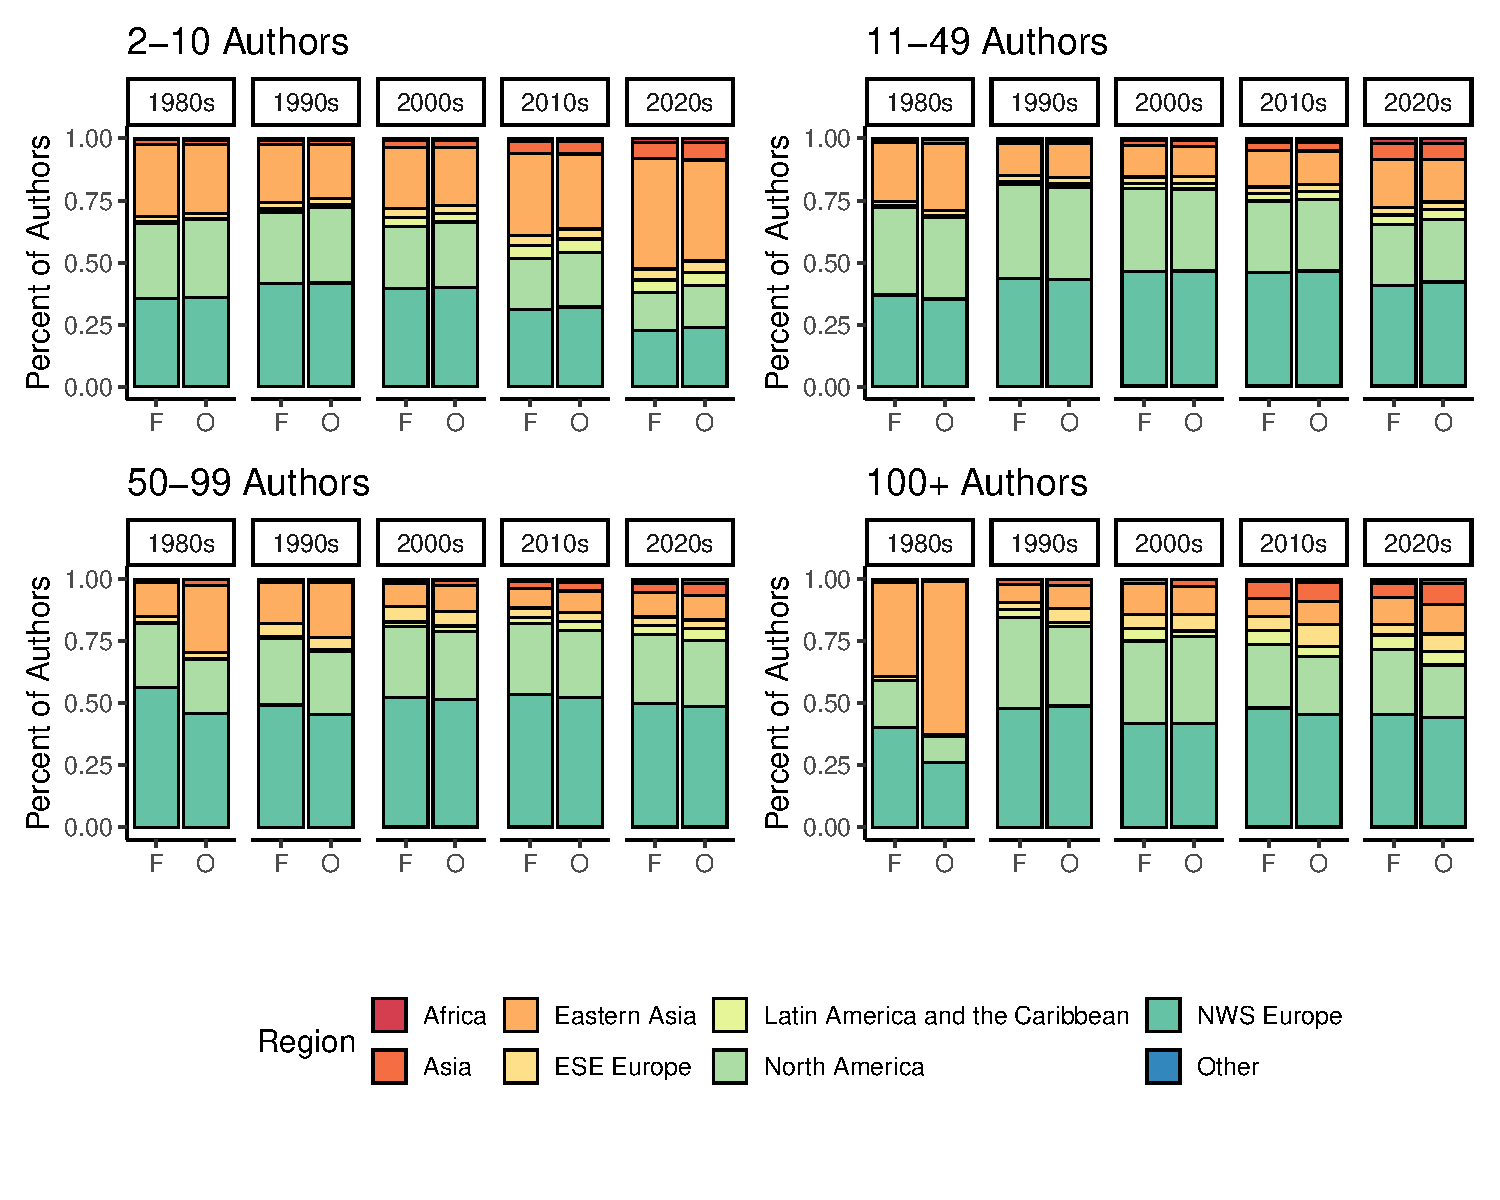
\includegraphics[keepaspectratio]{manuscript_definition_files/figure-latex/fig-author-gpe-1.pdf}}
\caption{\label{fig:fig-author-gpe}A comparison of author affiliation geopolitical regions across decades. F stands for first authors and O stands for other authors.}
\end{figure}

Across all decades and team sizes, North America and Northwestern Europe
consistently made up the majority of corresponding authors, as shown in
Figure \ref{fig:fig-author-gpe}. This pattern held even as total
team size increased, though the proportion of corresponding authors from
other regions (e.g., Asia, Latin America and the Caribbean, and Africa)
showed gradual increases over time. For traditional team science (2--10
authors), the dominance of North America and Western Europe in
corresponding author roles was particularly pronounced. In contrast, for
very large teams (100+ authors), regional diversity appeared somewhat
more balanced, with more visible contributions from Asia and other
regions among both corresponding and non-corresponding authors. However,
visual inspection suggests that corresponding author sets remained less
regionally diverse than the rest of the author team, particularly in
earlier decades. While representation from regions like Africa and Latin
America grew slightly among non-corresponding authors, they remained
minimally represented in lead authorship positions. Notably, Eastern
Asia's representation increased more substantially over time, especially
in teams with 50 or more authors. These visual trends suggest persistent
regional disparities in leadership roles within scientific publications,
despite increasing global collaboration. Quantitative effect sizes
(Cramer's \emph{V}) and confidence intervals are reported in the following
section to determine the importance of these observed differences.

Supplemental Figure \ref{fig:fig-effect-gpe} shows the magnitude of the difference in
regional representation between corresponding authors and all other
authors over time. A value of zero would indicate perfectly balanced
regional diversity between the two groups, whereas larger values reflect
increasing skew toward certain regions being more prominent in lead
authorship positions. Effect sizes were often non-zero across much of
the time span, particularly in publications with larger team sizes.
Papers with 50--99 authors and 100+ authors showed the highest effect
sizes in the 1970s through the 1990s, with \emph{V} values frequently
exceeding .20. This suggests that early large-team collaborations were
especially likely to concentrate lead authorship within a narrow set of
regions. However, across all team sizes, there was a clear downward
trend in effect sizes over time, indicating that the regional
composition of corresponding authors has become more similar to the rest
of the author team. In recent decades, effect sizes for team science and
mid-sized BTS teams (11--49 authors) have generally remained below 0.05,
suggesting relatively balanced representation. For larger teams, effect
sizes have also decreased, although they remain slightly elevated in
more recent years compared to smaller teams. As a reference for
interpretation, the vast majority of observed effects were small:
49.52\% of
comparisons had \(V\) \textless{} .05,
78.57\% had \(V\) \textless{}
.10, and 92.38\%
had \(V\) \textless{} .20. These results suggest that while regional imbalances in
leadership authorship persist, they have gradually diminished in
magnitude over time.

\section{Discussion}\label{discussion}

This study expands on prior efforts to characterize Big Team Science
(BTS) by providing a systematic, field-wide analysis of authorship
composition across time, team size, and geography. While BTS efforts
have been increasingly promoted as vehicles for collaboration, scale,
and rigor (Adams, 2012; Uhlmann et al., 2019), questions remain about who gets
included, who leads, and how equitably credit is distributed. A key
contribution of our study is that it is the first to propose a
data-driven operationalization of ``big'' teams: defined here as
publications with 11 or more authors and contributions from at least 6
institutions, grounded in the empirical distribution of team sizes and
affiliations across millions of papers. By comparing BTS publications
with traditional team science publications across four major scientific domains, we
clarify how BTS compares with traditional team science and how it is
evolving. All areas of research show growth in the number of
publications and authors included on manuscripts, replicating previous
investigations (Hunter \& Leahey, 2008; Sinatra et al., 2015; Wuchty et al., 2007).

Next, we find that early-career researchers are increasingly represented
in both BTS and smaller teams. Across all disciplines, the average
career length of authors decreased significantly over time. Traditional team science exhibited even steeper declines in both average and variability of
career length than big teams, suggesting that smaller teams may be an
especially important entry point for early-career researchers. These
trends echo broader shifts in academia's incentive structures, where
publishing early and often is increasingly required for career
advancement (Larivière et al., 2015; Milojević, 2014). Publication counts showed
similar but smaller effects. The average number of publications per
author declined over time in both big and small teams, with smaller
teams again showing more pronounced shifts. These findings support
claims that collaborative science is no longer dominated exclusively by
elite or high-output researchers (Milojević, 2014), but may instead be
expanding to include contributors with more varied publication
histories.

Our findings build on previous research by also examining diversity in
author seniority and geopolitical affiliation. The growing participation
of early-career scholars over time suggests that big team science may be
increasingly accessible to a broader range of researchers, not just
senior or established scientists. This trend is interesting given the
challenges BTS projects can pose for non-permanent researchers: slow
publication timelines, uncertain publication outcomes, and fewer
incentives for non-corresponding authors. Yet, large teams may allow for
more distributed workloads and reduced individual time investment, which
could make them appealing even for early-career researchers. Moreover,
prior work has shown that publications from larger teams tend to receive
more citations and have broader impact (Larivière et al., 2015), which may
further incentivize early-career involvement despite the structural
risks. Globalization, the internet, and the focus on interdisciplinary
research are potentially driving forces behind our results, but,
hopefully, the results also point to a decline in scientific gate keeping
(Lu, 2007; Siler et al., 2015).

Our results confirm and extend prior observations that both traditional team science
and BTS are disproportionately concentrated in high-resource, highly
networked regions, namely, North America and Western Europe (Adams, 2012; Singh et al., 2023; Sugimoto et al., 2017). However, this study offers a more nuanced
picture. We observed modest increases in the geographic diversity of
authorship. Yet, lead authorship remained concentrated in a relatively
narrow set of regions. These findings parallel previous critiques of
global equity in scientific collaboration, where authors from the Global
South are often included in co-authorship lists but remain
underrepresented in leadership roles (Chan et al., 2011; Sumathipala et al., 2004).
Though Cramer's \emph{V} values reflecting geographic imbalance decreased
over time, especially for small and mid-sized teams, some asymmetries
persist in large teams, reinforcing concerns about exclusion even within
globally scoped research efforts (Abimbola, 2019).

Diverse teams are more likely to produce research with stronger impact,
as reflected in higher citation metrics and broader dissemination,
particularly when author lists include individuals from varied
backgrounds and institutions (Freeman \& Huang, 2014; B. F. Jones et al., 2008; Yang et al., 2022).
These patterns underscore a broader shift in how scholarly contributions
are valued and attributed. As scientific teams become larger and more
interdisciplinary, traditional authorship conventions, especially the
emphasis on first and last author positions, become less informative
indicators of individual contribution (Allen et al., 2019; Brand et al., 2015). In
response, initiatives like the CRediT taxonomy have emerged to increase
transparency around contributor roles (Allen et al., 2014). Our findings
reinforce the importance of such systems: as early-career and
less-published researchers increasingly participate in both BTS and
regular teams, formal recognition of diverse contributions becomes
essential for equitable credit and career advancement.

The limitations for this research are tied to the curation of the Scopus
dataset: the correct author affiliations, the correct author publication
information, and the correctly marked geopolitical entity. Scopus is a
carefully curated and large dataset, but these limitations must be kept
in mind when interpreting the results. Publication language diversity
was not investigated, and a previous study indicates that most
publications in big databases are in English (Albarillo, 2014).
Certainly, publications in non-English languages would improve the
statistics on diversity in scientific publishing - but the English
language barrier likely exists regardless of inclusion in databases
(Meneghini \& Packer, 2007; Ramírez-Castañeda, 2020). Another limitation is the process of indexing across time has significantly changed with the availability of the internet. For example, in Figure \ref{fig:fig-paper-time}, traditional team science papers show a bump in the number of publications around approximately 1995, and the Web of Science came online in 1997, which included back indexing of journals not previous indexed.

Taken together, our findings suggest that BTS is evolving to include a
broader and more diverse range of contributors, but also that smaller
teams may remain more flexible or inclusive in incorporating
early-career and globally distributed researchers. This result carries
important implications for funders and institutions encouraging
large-scale collaboration. Without structural support for equitable
leadership, credit, and inclusion, particularly for authors from
underrepresented regions, BTS risks reinforcing the very hierarchies it
seeks to eliminate (Forscher et al., 2022).

\newpage

\section{References}\label{references}

\phantomsection\label{refs}
\begin{CSLReferences}{1}{0}
\bibitem[\citeproctext]{ref-aphilos2021}
A philosophical case for big physics. (2021). \emph{Nature Physics}, \emph{17}(6), 661--661. \url{https://doi.org/10.1038/s41567-021-01278-0}

\bibitem[\citeproctext]{ref-abimbola2019}
Abimbola, S. (2019). The foreign gaze: authorship in academic global health. \emph{BMJ Global Health}, \emph{4}(5). \url{https://doi.org/10.1136/bmjgh-2019-002068}

\bibitem[\citeproctext]{ref-adams2012}
Adams, J. (2012). The rise of research networks. \emph{Nature}, \emph{490}(7420), 335--336. \url{https://doi.org/10.1038/490335a}

\bibitem[\citeproctext]{ref-albarillo2014}
Albarillo, F. (2014). Language in social science databases: English versus non-english articles in JSTOR and scopus. \emph{Behavioral \& Social Sciences Librarian}, \emph{33}(2), 77--90. \url{https://doi.org/10.1080/01639269.2014.904693}

\bibitem[\citeproctext]{ref-allen2019}
Allen, L., O'Connell, A., \& Kiermer, V. (2019). How can we ensure visibility and diversity in research contributions? How the Contributor Role Taxonomy (CRediT) is helping the shift from authorship to contributorship. \emph{Learned Publishing}, \emph{32}(1), 71--74. \url{https://doi.org/10.1002/leap.1210}

\bibitem[\citeproctext]{ref-allen2014}
Allen, L., Scott, J., Brand, A., Hlava, M., \& Altman, M. (2014). Publishing: Credit where credit is due. \emph{Nature}, \emph{508}(7496), 312--313. \url{https://doi.org/10.1038/508312a}

\bibitem[\citeproctext]{ref-auspurg2021}
Auspurg, K., \& Brüderl, J. (2021). Has the Credibility of the Social Sciences Been Credibly Destroyed? Reanalyzing the {``}Many Analysts, One Data Set{''} Project. \emph{Socius: Sociological Research for a Dynamic World}, \emph{7}. \url{https://doi.org/10.1177/23780231211024421}

\bibitem[\citeproctext]{ref-bago2022}
Bago, B., Kovacs, M., Protzko, J., Nagy, T., Kekecs, Z., Palfi, B., Adamkovic, M., Adamus, S., Albalooshi, S., Albayrak-Aydemir, N., Alfian, I. N., Alper, S., Alvarez-Solas, S., Alves, S. G., Amaya, S., Andresen, P. K., Anjum, G., Ansari, D., Arriaga, P., \ldots{} Aczel, B. (2022). Situational factors shape moral judgements in the trolley dilemma in Eastern, Southern and Western countries in a culturally diverse sample. \emph{Nature Human Behaviour}, \emph{6}, 880--895. \url{https://doi.org/10.1038/s41562-022-01319-5}

\bibitem[\citeproctext]{ref-brand2015}
Brand, A., Allen, L., Altman, M., Hlava, M., \& Scott, J. (2015). Beyond authorship: attribution, contribution, collaboration, and credit. \emph{Learned Publishing}, \emph{28}(2), 151--155. \url{https://doi.org/10.1087/20150211}

\bibitem[\citeproctext]{ref-buchanan2023}
Buchanan, E. M., Lewis, S. C., Paris, B., Forscher, P. S., Pavlacic, J. M., Beshears, J. E., Drexler, S. M., Gourdon-Kanhukamwe, A., Mallik, P. R., Silan, M. A. A., Miller, J. K., IJzerman, H., Moshontz, H., Beaudry, J. L., Suchow, J. W., Chartier, C. R., Coles, N. A., Sharifian, M., Todsen, A. L., \ldots{} McFall, J. P. (2023). The psychological science accelerator{'}s COVID-19 rapid-response dataset. \emph{Scientific Data}, \emph{10}(1), 87. \url{https://doi.org/10.1038/s41597-022-01811-7}

\bibitem[\citeproctext]{ref-buttrick2020}
Buttrick, N. R., Aczel, B., Aeschbach, L. F., Bakos, B. E., Brühlmann, F., Claypool, H. M., Hüffmeier, J., Kovacs, M., Schuepfer, K., Szecsi, P., Szuts, A., Szöke, O., Thomae, M., Torka, A.-K., Walker, R. J., \& Wood, M. J. (2020). Many Labs 5: Registered Replication of Vohs and Schooler (2008), Experiment 1. \emph{Advances in Methods and Practices in Psychological Science}, \emph{3}(3), 429--438. \url{https://doi.org/10.1177/2515245920917931}

\bibitem[\citeproctext]{ref-castelnovo2018}
Castelnovo, P., Florio, M., Forte, S., Rossi, L., \& Sirtori, E. (2018). The economic impact of technological procurement for large-scale research infrastructures: Evidence from the Large Hadron Collider at CERN. \emph{Research Policy}, \emph{47}(9), 1853--1867. \url{https://doi.org/10.1016/j.respol.2018.06.018}

\bibitem[\citeproctext]{ref-chan2011}
Chan, L., Kirsop, B., \& Arunachalam, S. (2011). Towards Open and Equitable Access to Research and Knowledge for Development. \emph{PLoS Medicine}, \emph{8}(3), e1001016. \url{https://doi.org/10.1371/journal.pmed.1001016}

\bibitem[\citeproctext]{ref-coles2022}
Coles, N. A., Hamlin, J. K., Sullivan, L. L., Parker, T. H., \& Altschul, D. (2022). Build up big-team science. \emph{Nature}, \emph{601}(7894), 505--507. \url{https://doi.org/10.1038/d41586-022-00150-2}

\bibitem[\citeproctext]{ref-collins2003}
Collins, F. S., Morgan, M., \& Patrinos, A. (2003). The human genome project: Lessons from large-scale biology. \emph{Science}, \emph{300}(5617), 286--290. \url{https://doi.org/10.1126/science.1084564}

\bibitem[\citeproctext]{ref-council2015}
Council, N. R., Education, D. of B., Sciences, S., Sciences, B. on B. C. and S. and, \& Science, C. on the S. of T. (2015). \emph{Enhancing the Effectiveness of Team Science}. National Academies Press.

\bibitem[\citeproctext]{ref-cummings2007}
Cummings, J. N., \& Kiesler, S. (2007). Coordination costs and project outcomes in multi-university collaborations. \emph{Research Policy}, \emph{36}(10), 1620--1634. \url{https://doi.org/10.1016/j.respol.2007.09.001}

\bibitem[\citeproctext]{ref-dorison2022}
Dorison, C. A., Lerner, J. S., Heller, B. H., Rothman, A. J., Kawachi, I. I., Wang, K., Rees, V. W., Gill, B. P., Gibbs, N., Ebersole, C. R., Vally, Z., Tajchman, Z., Zsido, A. N., Zrimsek, M., Chen, Z., Ziano, I., Gialitaki, Z., Ceary, C. D., Lin, Y., \ldots{} Coles, N. A. (2022). In {COVID}-19 {Health} {Messaging}, {Loss} {Framing} {Increases} {Anxiety} with {Little}-to-{No} {Concomitant} {Benefits}: {Experimental} {Evidence} from 84 {Countries}. \emph{Affective Science}, \emph{3}(3), 577--602. \url{https://doi.org/10.1007/s42761-022-00128-3}

\bibitem[\citeproctext]{ref-ebersole2016}
Ebersole, C. R., Atherton, O. E., Belanger, A. L., Skulborstad, H. M., Allen, J. M., Banks, J. B., Baranski, E., Bernstein, M. J., Bonfiglio, D. B. V., Boucher, L., Brown, E. R., Budiman, N. I., Cairo, A. H., Capaldi, C. A., Chartier, C. R., Chung, J. M., Cicero, D. C., Coleman, J. A., Conway, J. G., \ldots{} Nosek, B. A. (2016). Many Labs 3: Evaluating participant pool quality across the academic semester via replication. \emph{Journal of Experimental Social Psychology}, \emph{67}, 68--82. \url{https://doi.org/10.1016/j.jesp.2015.10.012}

\bibitem[\citeproctext]{ref-ebersole2020}
Ebersole, C. R., Mathur, M. B., Baranski, E., Bart-Plange, D.-J., Buttrick, N. R., Chartier, C. R., Corker, K. S., Corley, M., Hartshorne, J. K., IJzerman, H., Lazarević, L. B., Rabagliati, H., Ropovik, I., Aczel, B., Aeschbach, L. F., Andrighetto, L., Arnal, J. D., Arrow, H., Babincak, P., \ldots{} Nosek, B. A. (2020). Many Labs 5: Testing Pre-Data-Collection Peer Review as an Intervention to Increase Replicability. \emph{Advances in Methods and Practices in Psychological Science}, \emph{3}(3), 309--331. \url{https://doi.org/10.1177/2515245920958687}

\bibitem[\citeproctext]{ref-elzhov2023}
Elzhov, T. V., Mullen, K. M., Spiess, A.-N., \& Bolker, B. (2023). \emph{Minpack.lm: R interface to the levenberg-marquardt nonlinear least-squares algorithm found in MINPACK, plus support for bounds}. \url{https://cran.r-project.org/web/packages/minpack.lm/index.html}

\bibitem[\citeproctext]{ref-10.7554ux2feLife.71601}
Errington, T. M., Mathur, M., Soderberg, C. K., Denis, A., Perfito, N., Iorns, E., \& Nosek, B. A. (2021). Investigating the replicability of preclinical cancer biology. \emph{eLife}, \emph{10}, e71601. \url{https://doi.org/10.7554/eLife.71601}

\bibitem[\citeproctext]{ref-fiore2008}
Fiore, S. M. (2008). Interdisciplinarity as Teamwork: How the Science of Teams Can Inform Team Science. \emph{Small Group Research}, \emph{39}(3), 251--277. \url{https://doi.org/10.1177/1046496408317797}

\bibitem[\citeproctext]{ref-forscher2022a}
Forscher, P. S., Wagenmakers, E.-J., Coles, N. A., Silan, M. A., Dutra, N., Basnight-Brown, D., \& IJzerman, H. (2022). The Benefits, Barriers, and Risks of Big-Team Science. \emph{Perspectives on Psychological Science}, \emph{18}(3), 607623. \url{https://doi.org/10.1177/17456916221082970}

\bibitem[\citeproctext]{ref-freeman2014}
Freeman, R. B., \& Huang, W. (2014). Collaboration: Strength in diversity. \emph{Nature}, \emph{513}(7518), 305--305. \url{https://doi.org/10.1038/513305a}

\bibitem[\citeproctext]{ref-grahe2014}
Grahe, J. E. (2014). Announcing open science badges and reaching for the sky. \emph{The Journal of Social Psychology}, \emph{154}(1), 1--3. \url{https://doi.org/10.1080/00224545.2014.853582}

\bibitem[\citeproctext]{ref-henrich2010}
Henrich, J., Heine, S. J., \& Norenzayan, A. (2010). The weirdest people in the world? \emph{Behavioral and Brain Sciences}, \emph{33}(2-3), 61--83. \url{https://doi.org/10.1017/S0140525X0999152X}

\bibitem[\citeproctext]{ref-hunter2008}
Hunter, L., \& Leahey, E. (2008). Collaborative Research in Sociology: Trends and Contributing Factors. \emph{The American Sociologist}, \emph{39}(4), 290--306. \url{https://doi.org/10.1007/s12108-008-9042-1}

\bibitem[\citeproctext]{ref-john2012}
John, L. K., Loewenstein, G., \& Prelec, D. (2012). Measuring the Prevalence of Questionable Research Practices With Incentives for Truth Telling. \emph{Psychological Science}, \emph{23}(5), 524--532. \url{https://doi.org/10.1177/0956797611430953}

\bibitem[\citeproctext]{ref-jones2021}
Jones, B. C., DeBruine, L. M., Flake, J. K., Liuzza, M. T., Antfolk, J., Arinze, N. C., Ndukaihe, I. L. G., Bloxsom, N. G., Lewis, S. C., Foroni, F., Willis, M. L., Cubillas, C. P., Vadillo, M. A., Turiegano, E., Gilead, M., Simchon, A., Saribay, S. A., Owsley, N. C., Jang, C., \ldots{} Coles, N. A. (2021). To which world regions does the valence{\textendash}dominance model of social perception apply? \emph{Nature Human Behaviour}, \emph{5}(1), 159--169. \url{https://doi.org/10.1038/s41562-020-01007-2}

\bibitem[\citeproctext]{ref-jones2008}
Jones, B. F., Wuchty, S., \& Uzzi, B. (2008). Multi-university research teams: Shifting impact, geography, and stratification in science. \emph{Science}, \emph{322}(5905), 1259--1262. \url{https://doi.org/10.1126/science.1158357}

\bibitem[\citeproctext]{ref-kidwell2016}
Kidwell, M. C., Lazarević, L. B., Baranski, E., Hardwicke, T. E., Piechowski, S., Falkenberg, L.-S., Kennett, C., Slowik, A., Sonnleitner, C., Hess-Holden, C., Errington, T. M., Fiedler, S., \& Nosek, B. A. (2016). Badges to Acknowledge Open Practices: A Simple, Low-Cost, Effective Method for Increasing Transparency. \emph{PLOS Biology}, \emph{14}(5), e1002456. \url{https://doi.org/10.1371/journal.pbio.1002456}

\bibitem[\citeproctext]{ref-klein2022}
Klein, R. A., Cook, C. L., Ebersole, C. R., Vitiello, C., Nosek, B. A., Hilgard, J., Ahn, P. H., Brady, A. J., Chartier, C. R., Christopherson, C. D., Clay, S., Collisson, B., Crawford, J. T., Cromar, R., Gardiner, G., Gosnell, C. L., Grahe, J., Hall, C., Howard, I., \ldots{} Ratliff, K. A. (2022). Many Labs 4: Failure to Replicate Mortality Salience Effect With and Without Original Author Involvement. \emph{Collabra: Psychology}, \emph{8}(1), 35271. \url{https://doi.org/10.1525/collabra.35271}

\bibitem[\citeproctext]{ref-klein2018}
Klein, R. A., Vianello, M., Hasselman, F., Adams, B. G., Adams, R. B., Alper, S., Aveyard, M., Axt, J. R., Babalola, M. T., Bahník, Š., Batra, R., Berkics, M., Bernstein, M. J., Berry, D. R., Bialobrzeska, O., Binan, E. D., Bocian, K., Brandt, M. J., Busching, R., \ldots{} Nosek, B. A. (2018). Many Labs 2: Investigating Variation in Replicability Across Samples and Settings. \emph{Advances in Methods and Practices in Psychological Science}, \emph{1}(4), 443--490. \url{https://doi.org/10.1177/2515245918810225}

\bibitem[\citeproctext]{ref-lariviuxe8re2015}
Larivière, V., Gingras, Y., Sugimoto, C. R., \& Tsou, A. (2015). Team size matters: Collaboration and scientific impact since 1900. \emph{Journal of the Association for Information Science and Technology}, \emph{66}(7), 1323--1332. \url{https://doi.org/10.1002/asi.23266}

\bibitem[\citeproctext]{ref-lebel2018}
LeBel, E. P., McCarthy, R. J., Earp, B. D., Elson, M., \& Vanpaemel, W. (2018). A Unified Framework to Quantify the Credibility of Scientific Findings. \emph{Advances in Methods and Practices in Psychological Science}, \emph{1}(3), 389--402. \url{https://doi.org/10.1177/2515245918787489}

\bibitem[\citeproctext]{ref-lu2007}
Lu, Y. (2007). The human in human information acquisition: Understanding gatekeeping and proposing new directions in scholarship. \emph{Library \& Information Science Research}, \emph{29}(1), 103--123. \url{https://doi.org/10.1016/j.lisr.2006.10.007}

\bibitem[\citeproctext]{ref-mathur2020}
Mathur, M. B., Bart-Plange, D.-J., Aczel, B., Bernstein, M. H., Ciunci, A. M., Ebersole, C. R., Falcão, F., Ashbaugh, K., Hilliard, R. A., Jern, A., Kellier, D. J., Kessinger, G., Kolb, V. S., Kovacs, M., Lage, C. A., Langford, E. V., Lins, S., Manfredi, D., Meyet, V., \ldots{} Frank, M. C. (2020). Many Labs 5: Registered Multisite Replication of the Tempting-Fate Effects in Risen and Gilovich (2008). \emph{Advances in Methods and Practices in Psychological Science}, \emph{3}(3), 394--404. \url{https://doi.org/10.1177/2515245918785165}

\bibitem[\citeproctext]{ref-maxwell2015}
Maxwell, S. E., Lau, M. Y., \& Howard, G. S. (2015). Is psychology suffering from a replication crisis?: What does 'failure to replicate' really mean? \emph{American Psychologist}, \emph{70}(6), 487--498. \url{https://doi.org/10.1037/a0039400}

\bibitem[\citeproctext]{ref-mayo-wilson2021}
Mayo-Wilson, E., Grant, S., Supplee, L., Kianersi, S., Amin, A., DeHaven, A., \& Mellor, D. (2021). Evaluating implementation of the transparency and openness promotion~(TOP) guidelines:~The TRUST process for rating journal policies, procedures, and practices. \emph{Research Integrity and Peer Review}, \emph{6}(1), 9. \url{https://doi.org/10.1186/s41073-021-00112-8}

\bibitem[\citeproctext]{ref-meneghini2007}
Meneghini, R., \& Packer, A. L. (2007). Is there science beyond english? \emph{EMBO Reports}, \emph{8}(2), 112--116. \url{https://doi.org/10.1038/sj.embor.7400906}

\bibitem[\citeproctext]{ref-milojevic2014}
Milojević, S. (2014). Principles of scientific research team formation and evolution. \emph{Proceedings of the National Academy of Sciences}, \emph{111}(11), 3984--3989. \url{https://doi.org/10.1073/pnas.1309723111}

\bibitem[\citeproctext]{ref-moshontz2018}
Moshontz, H., Campbell, L., Ebersole, C. R., IJzerman, H., Urry, H. L., Forscher, P. S., Grahe, J. E., McCarthy, R. J., Musser, E. D., Antfolk, J., Castille, C. M., Evans, T. R., Fiedler, S., Flake, J. K., Forero, D. A., Janssen, S. M. J., Keene, J. R., Protzko, J., Aczel, B., \ldots{} Chartier, C. R. (2018). The Psychological Science Accelerator: Advancing Psychology Through a Distributed Collaborative Network. \emph{Advances in Methods and Practices in Psychological Science}, \emph{1}(4), 501--515. \url{https://doi.org/10.1177/2515245918797607}

\bibitem[\citeproctext]{ref-nelson2018}
Nelson, L. D., Simmons, J., \& Simonsohn, U. (2018). Psychology's renaissance. \emph{Annual Review of Psychology}, \emph{69}(1), 511--534. \url{https://doi.org/10.1146/annurev-psych-122216-011836}

\bibitem[\citeproctext]{ref-newson2021}
Newson, M., Buhrmester, M., Xygalatas, D., \& Whitehouse, H. (2021). Go WILD, not WEIRD. \emph{Journal for the Cognitive Science of Religion}, \emph{6}(1-2). \url{https://doi.org/10.1558/jcsr.38413}

\bibitem[\citeproctext]{ref-nosek2015}
Nosek, B. A., Alter, G., Banks, G. C., Borsboom, D., Bowman, S. D., Breckler, S. J., Buck, S., Chambers, C. D., Chin, G., Christensen, G., Contestabile, M., Dafoe, A., Eich, E., Freese, J., Glennerster, R., Goroff, D., Green, D. P., Hesse, B., Humphreys, M., \ldots{} Yarkoni, T. (2015). Promoting an open research culture. \emph{Science}, \emph{348}(6242), 1422--1425. \url{https://doi.org/10.1126/science.aab2374}

\bibitem[\citeproctext]{ref-nosek2014method}
Nosek, B. A., \& Lakens, D. (2014a). A method to increase the credibility of published results. \emph{Social Psychology}, \emph{45}(3), 137141.

\bibitem[\citeproctext]{ref-nosek2014}
Nosek, B. A., \& Lakens, D. (2014b). Registered Reports: A Method to Increase the Credibility of Published Results. \emph{Social Psychology}, \emph{45}(3), 137--141. \url{https://doi.org/10.1027/1864-9335/a000192}

\bibitem[\citeproctext]{ref-opensciencecollaboration2015}
Open Science Collaboration. (2015). Estimating the reproducibility of psychological science. \emph{Science}, \emph{349}(6251), aac4716--aac4716. \url{https://doi.org/10.1126/science.aac4716}

\bibitem[\citeproctext]{ref-psychologicalscienceacceleratorself-determinationtheorycollaboration2022}
Psychological Science Accelerator Self-Determination Theory Collaboration. (2022). A global experiment on motivating social distancing during the COVID-19 pandemic. \emph{Proceedings of the National Academy of Sciences}, \emph{119}(22), e2111091119. \url{https://doi.org/10.1073/pnas.2111091119}

\bibitem[\citeproctext]{ref-rad2018}
Rad, M. S., Martingano, A. J., \& Ginges, J. (2018). Toward a psychology of homo sapiens: Making psychological science more representative of the human population. \emph{Proceedings of the National Academy of Sciences}, \emph{115}(45), 11401--11405. \url{https://doi.org/10.1073/pnas.1721165115}

\bibitem[\citeproctext]{ref-ramuxedrez-castauxf1eda2020}
Ramírez-Castañeda, V. (2020). Disadvantages in preparing and publishing scientific papers caused by the dominance of the English language in science: The case of Colombian researchers in biological sciences. \emph{PLOS ONE}, \emph{15}(9), e0238372. \url{https://doi.org/10.1371/journal.pone.0238372}

\bibitem[\citeproctext]{ref-silberzahn2018many}
Silberzahn, R., Uhlmann, E. L., Martin, D. P., Anselmi, P., Aust, F., Awtrey, E., Bahník, Š., Bai, F., Bannard, C., Bonnier, E., \& others. (2018). Many analysts, one data set: Making transparent how variations in analytic choices affect results. \emph{Advances in Methods and Practices in Psychological Science}, \emph{1}(3), 337356.

\bibitem[\citeproctext]{ref-siler2015}
Siler, K., Lee, K., \& Bero, L. (2015). Measuring the effectiveness of scientific gatekeeping. \emph{Proceedings of the National Academy of Sciences}, \emph{112}(2), 360--365. \url{https://doi.org/10.1073/pnas.1418218112}

\bibitem[\citeproctext]{ref-sinatra2015}
Sinatra, R., Deville, P., Szell, M., Wang, D., \& Barabási, A.-L. (2015). A century of physics. \emph{Nature Physics}, \emph{11}(10), 791--796. \url{https://doi.org/10.1038/nphys3494}

\bibitem[\citeproctext]{ref-singh2023}
Singh, L., Killen, M., Smetana, \& G., J. (2023). Global Science Requires Greater Equity, Diversity, and Cultural Precision. \emph{APS Observer}, \emph{36}. \url{https://www.psychologicalscience.org/observer/gs-equity-diversity-cultural-precision}

\bibitem[\citeproctext]{ref-skorb2020}
Skorb, L., Aczel, B., Bakos, B. E., Feinberg, L., Hałasa, E., Kauff, M., Kovacs, M., Krasuska, K., Kuchno, K., Manfredi, D., Montealegre, A., Pękala, E., Pieńkosz, D., Ravid, J., Rentzsch, K., Szaszi, B., Schulz-Hardt, S., Sioma, B., Szecsi, P., \ldots{} Hartshorne, J. K. (2020). Many Labs 5: Replication of van Dijk, van Kleef, Steinel, and van Beest (2008). \emph{Advances in Methods and Practices in Psychological Science}, \emph{3}(3), 418--428. \url{https://doi.org/10.1177/2515245920927643}

\bibitem[\citeproctext]{ref-stewart2017}
Stewart, N., Chandler, J., \& Paolacci, G. (2017). Crowdsourcing samples in cognitive science. \emph{Trends in Cognitive Sciences}, \emph{21}(10), 736--748. \url{https://doi.org/10.1016/j.tics.2017.06.007}

\bibitem[\citeproctext]{ref-stewart2020}
Stewart, S., Rinke, E. M., McGarrigle, R., Lynott, D., Lunny, C., Lautarescu, A., Galizzi, M. M., Farran, E. K., \& Crook, Z. (2020). \emph{Pre-registration and registered reports: A primer from UKRN}. \url{https://doi.org/10.31219/osf.io/8v2n7}

\bibitem[\citeproctext]{ref-sugimoto2017}
Sugimoto, C. R., Robinson-Garcia, N., Murray, D. S., Yegros-Yegros, A., Costas, R., \& Larivière, V. (2017). Scientists have most impact when they're free to move. \emph{Nature}, \emph{550}(7674), 29--31. \url{https://doi.org/10.1038/550029a}

\bibitem[\citeproctext]{ref-sumathipala2004}
Sumathipala, A., Siribaddana, S., \& Patel, V. (2004). Under-representation of developing countries in the research literature: ethical issues arising from a survey of five leading medical journals. \emph{BMC Medical Ethics}, \emph{5}(1), 5. \url{https://doi.org/10.1186/1472-6939-5-5}

\bibitem[\citeproctext]{ref-uhlmann2019}
Uhlmann, E. L., Ebersole, C. R., Chartier, C. R., Errington, T. M., Kidwell, M. C., Lai, C. K., McCarthy, R. J., Riegelman, A., Silberzahn, R., \& Nosek, B. A. (2019). Scientific Utopia III: Crowdsourcing Science. \emph{Perspectives on Psychological Science}, \emph{14}(5), 711--733. \url{https://doi.org/10.1177/1745691619850561}

\bibitem[\citeproctext]{ref-vanbavel2022}
Van Bavel, J. J., Cichocka, A., Capraro, V., Sjåstad, H., Nezlek, J. B., Pavlović, T., Alfano, M., Gelfand, M. J., Azevedo, F., Birtel, M. D., Cislak, A., Lockwood, P. L., Ross, R. M., Abts, K., Agadullina, E., Aruta, J. J. B., Besharati, S. N., Bor, A., Choma, B. L., \ldots{} Boggio, P. S. (2022). National identity predicts public health support during a global pandemic. \emph{Nature Communications}, \emph{13}(1), 517. \url{https://doi.org/10.1038/s41467-021-27668-9}

\bibitem[\citeproctext]{ref-vazire2022}
Vazire, S., Schiavone, S. R., \& Bottesini, J. G. (2022). Credibility Beyond Replicability: Improving the Four Validities in Psychological Science. \emph{Current Directions in Psychological Science}, \emph{31}(2), 162--168. \url{https://doi.org/10.1177/09637214211067779}

\bibitem[\citeproctext]{ref-wang2021}
Wang, K., Goldenberg, A., Dorison, C. A., Miller, J. K., Uusberg, A., Lerner, J. S., Gross, J. J., Agesin, B. B., Bernardo, M., Campos, O., Eudave, L., Grzech, K., Ozery, D. H., Jackson, E. A., Garcia, E. O. L., Drexler, S. M., Jurković, A. P., Rana, K., Wilson, J. P., \ldots{} Moshontz, H. (2021). A multi-country test of brief reappraisal interventions on emotions during the COVID-19 pandemic. \emph{Nature Human Behaviour}, \emph{5}(8), 1089--1110. \url{https://doi.org/10.1038/s41562-021-01173-x}

\bibitem[\citeproctext]{ref-wickham2007}
Wickham, H. (2007). Reshaping Data with the reshape Package. \emph{Journal of Statistical Software}, \emph{21}(1), 1--20. \url{https://doi.org/10.18637/jss.v021.i12}

\bibitem[\citeproctext]{ref-wuchty2007}
Wuchty, S., Jones, B. F., \& Uzzi, B. (2007). The increasing dominance of teams in production of knowledge. \emph{Science}, \emph{316}(5827), 1036--1039. \url{https://doi.org/10.1126/science.1136099}

\bibitem[\citeproctext]{ref-yang2022}
Yang, Y., Tian, T. Y., Woodruff, T. K., Jones, B. F., \& Uzzi, B. (2022). Gender-diverse teams produce more novel and higher-impact scientific ideas. \emph{Proceedings of the National Academy of Sciences}, \emph{119}(36), e2200841119. \url{https://doi.org/10.1073/pnas.2200841119}

\bibitem[\citeproctext]{ref-zwaan2018}
Zwaan, R. A., Etz, A., Lucas, R. E., \& Donnellan, M. B. (2018). Making replication mainstream. \emph{Behavioral and Brain Sciences}, \emph{41}, e120. \url{https://doi.org/10.1017/S0140525X17001972}

\end{CSLReferences}

\newpage

\appendix


\section{Supplemental Material}\label{supplemental-material}

We have included several supplemental tables and figures for visualization of results discussed in the manuscript.

\begin{figure}
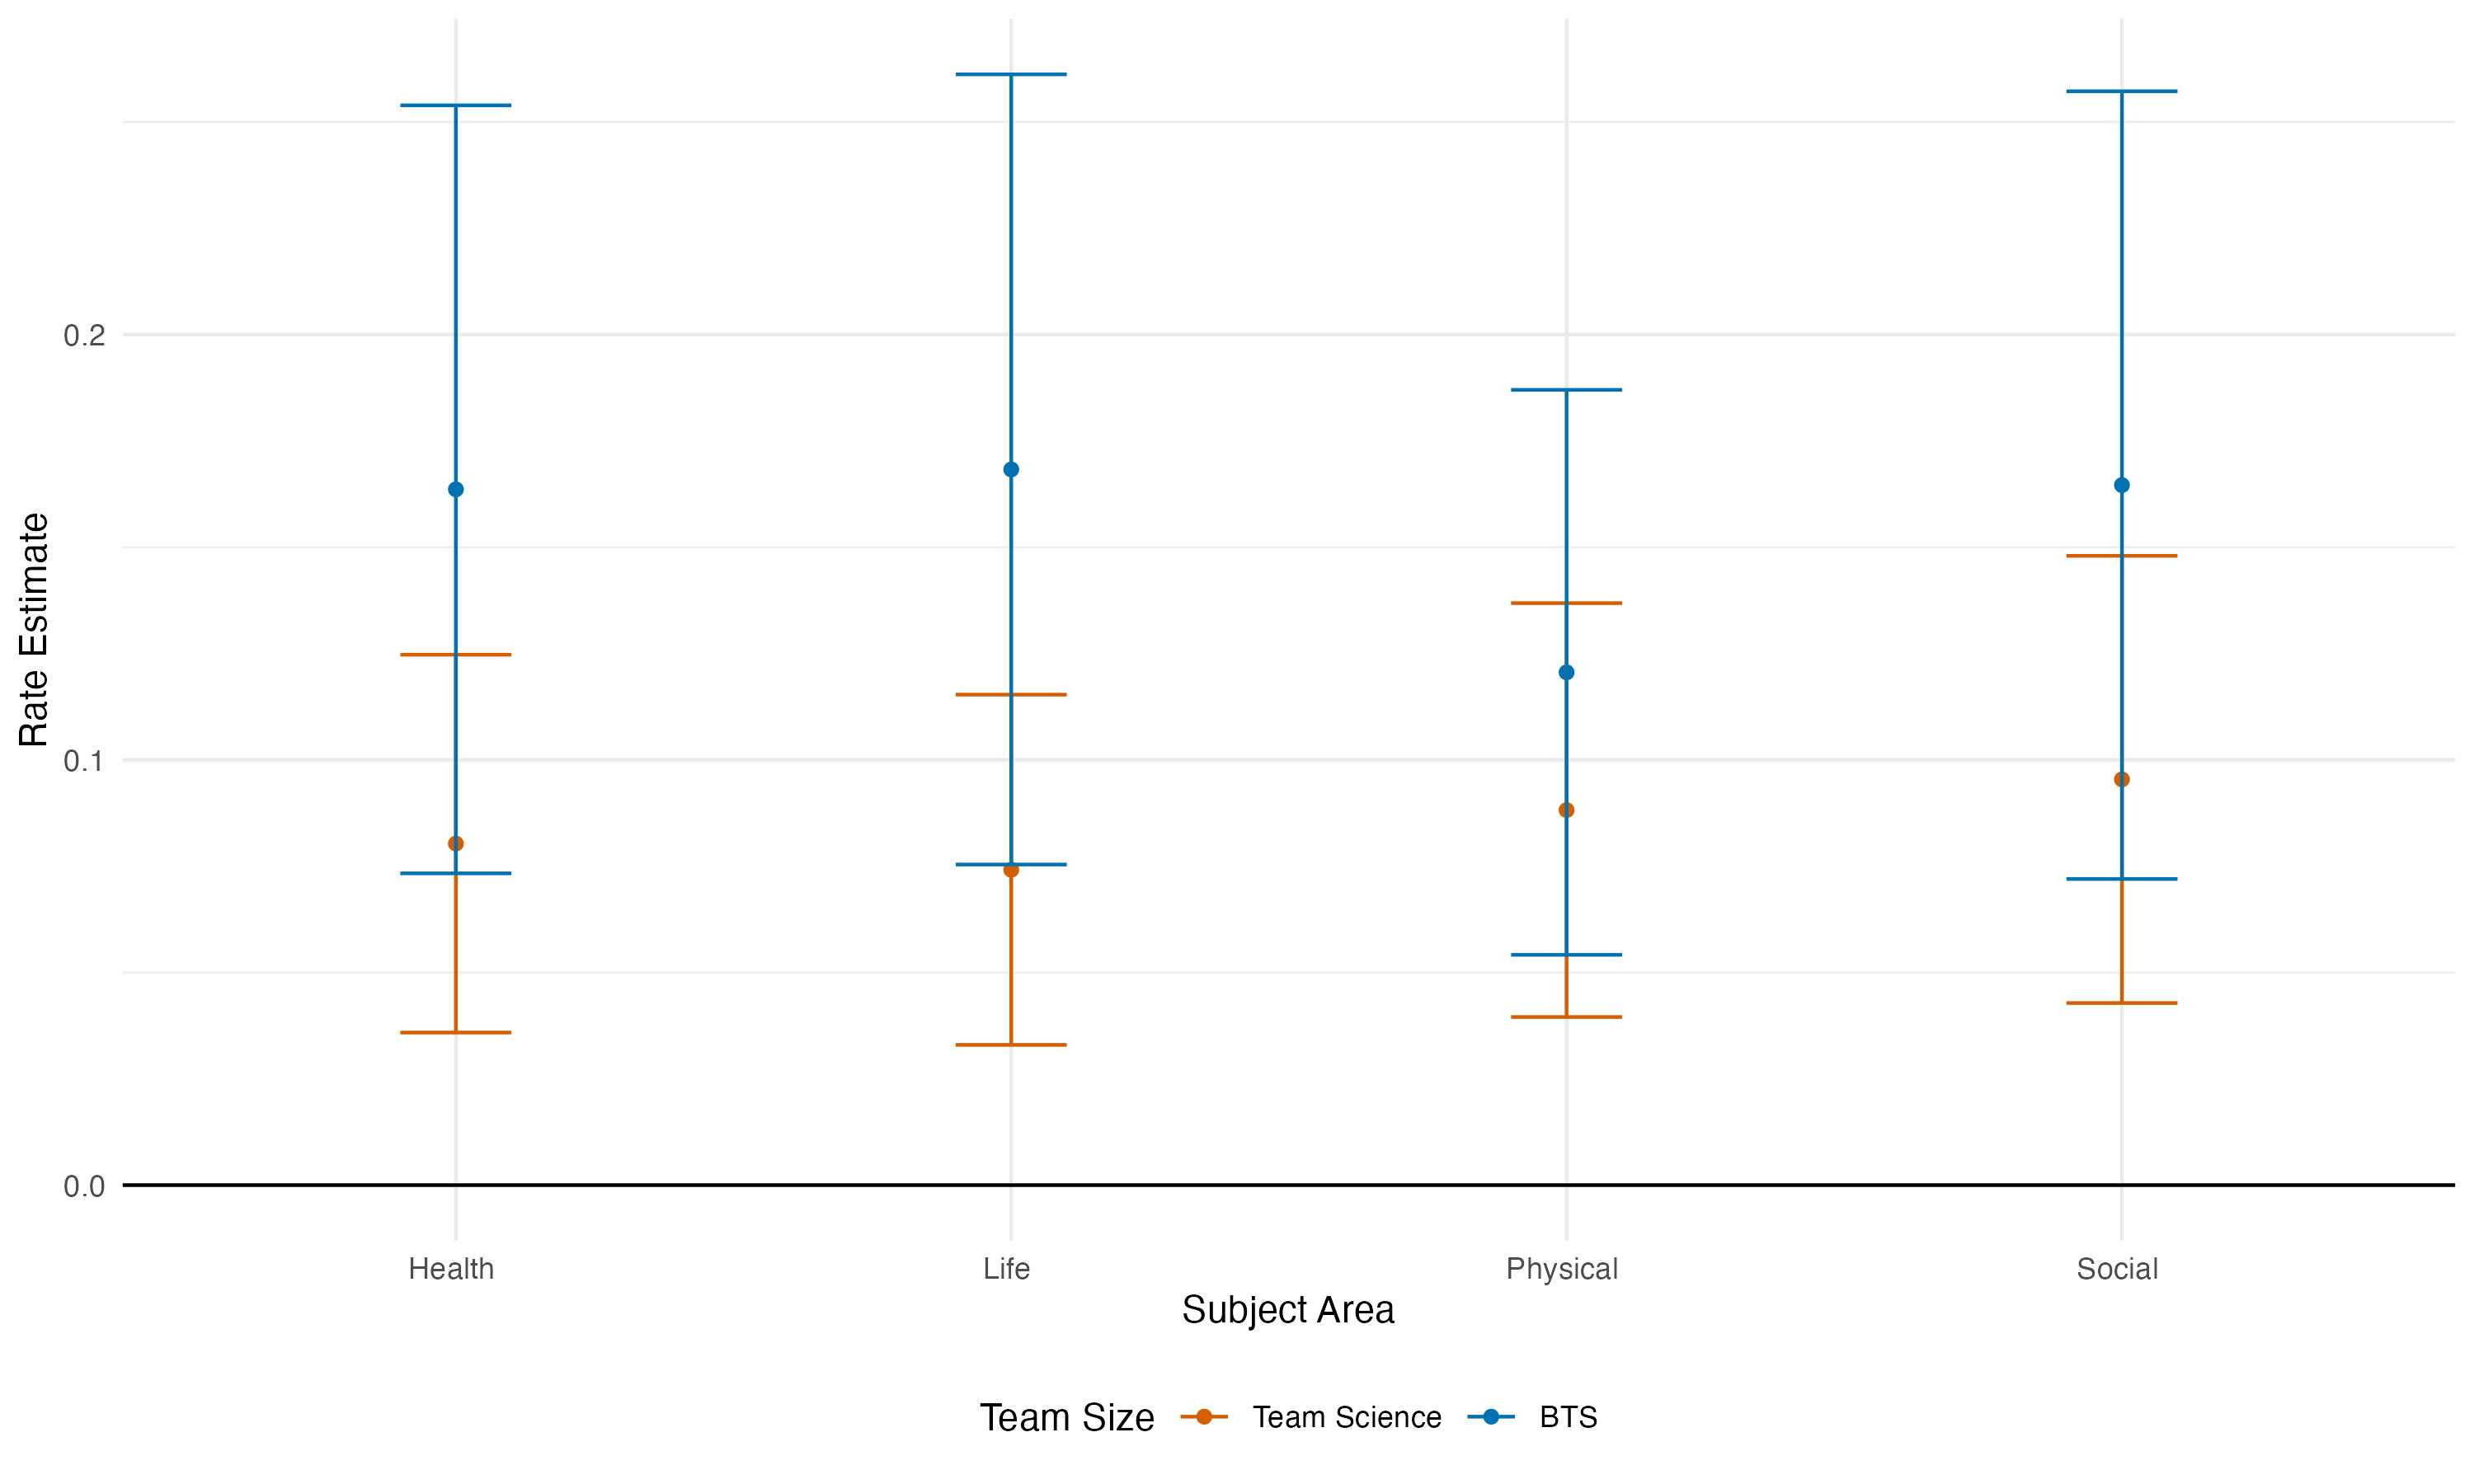
\includegraphics[width=1\linewidth]{figure/figure_3_growth} \caption{Exponential growth rate estimates with 95\% confidence intervals.}\label{fig:rate-estimates-fig}
\end{figure}

\begin{figure}
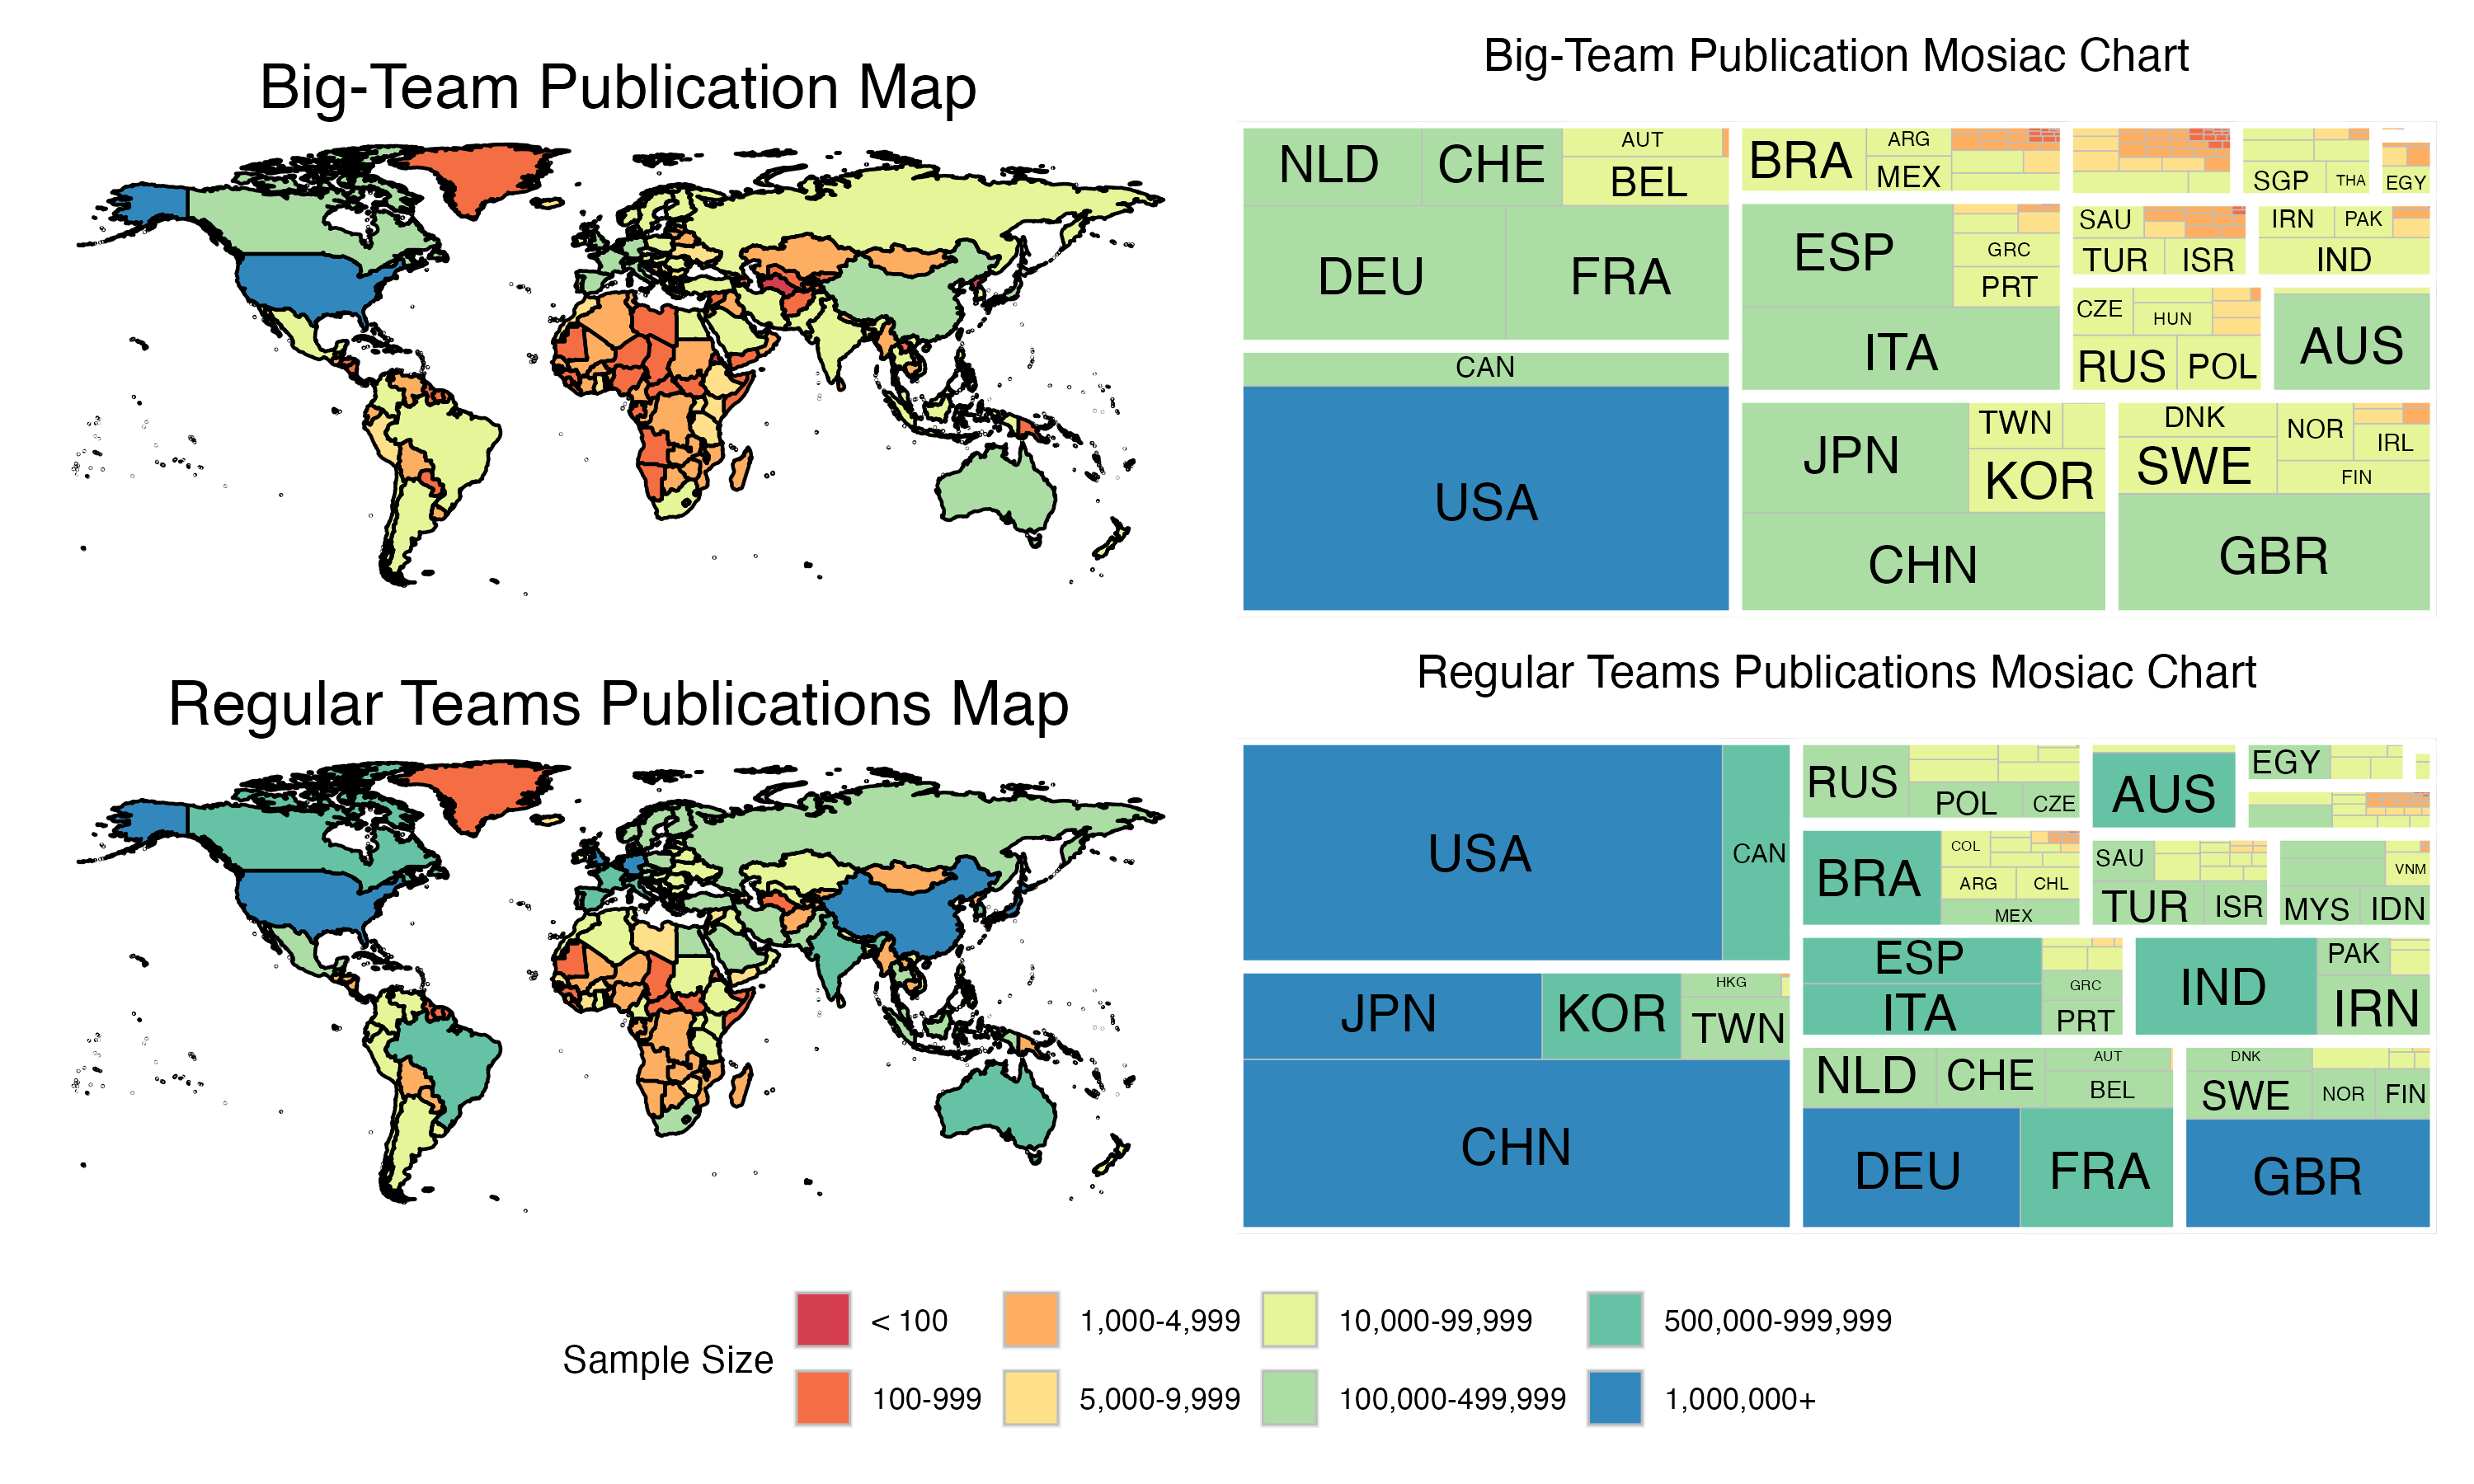
\includegraphics[width=1\linewidth]{figure/figure_6_map} \caption{Geopolitical regions represented in big-team science publications versus all publications. The mosaic plot is grouped by UN subregion with the largest number of publications starting on the bottom left and smallest on the top right. Therefore, North America represents the largest number of authors within BTS (i.e., bottom right, then separated into the geopolitical areas within that subregion), followed by Eastern Europe (top left), and so on.}\label{fig:fig-map-both}
\end{figure}

\begin{figure}
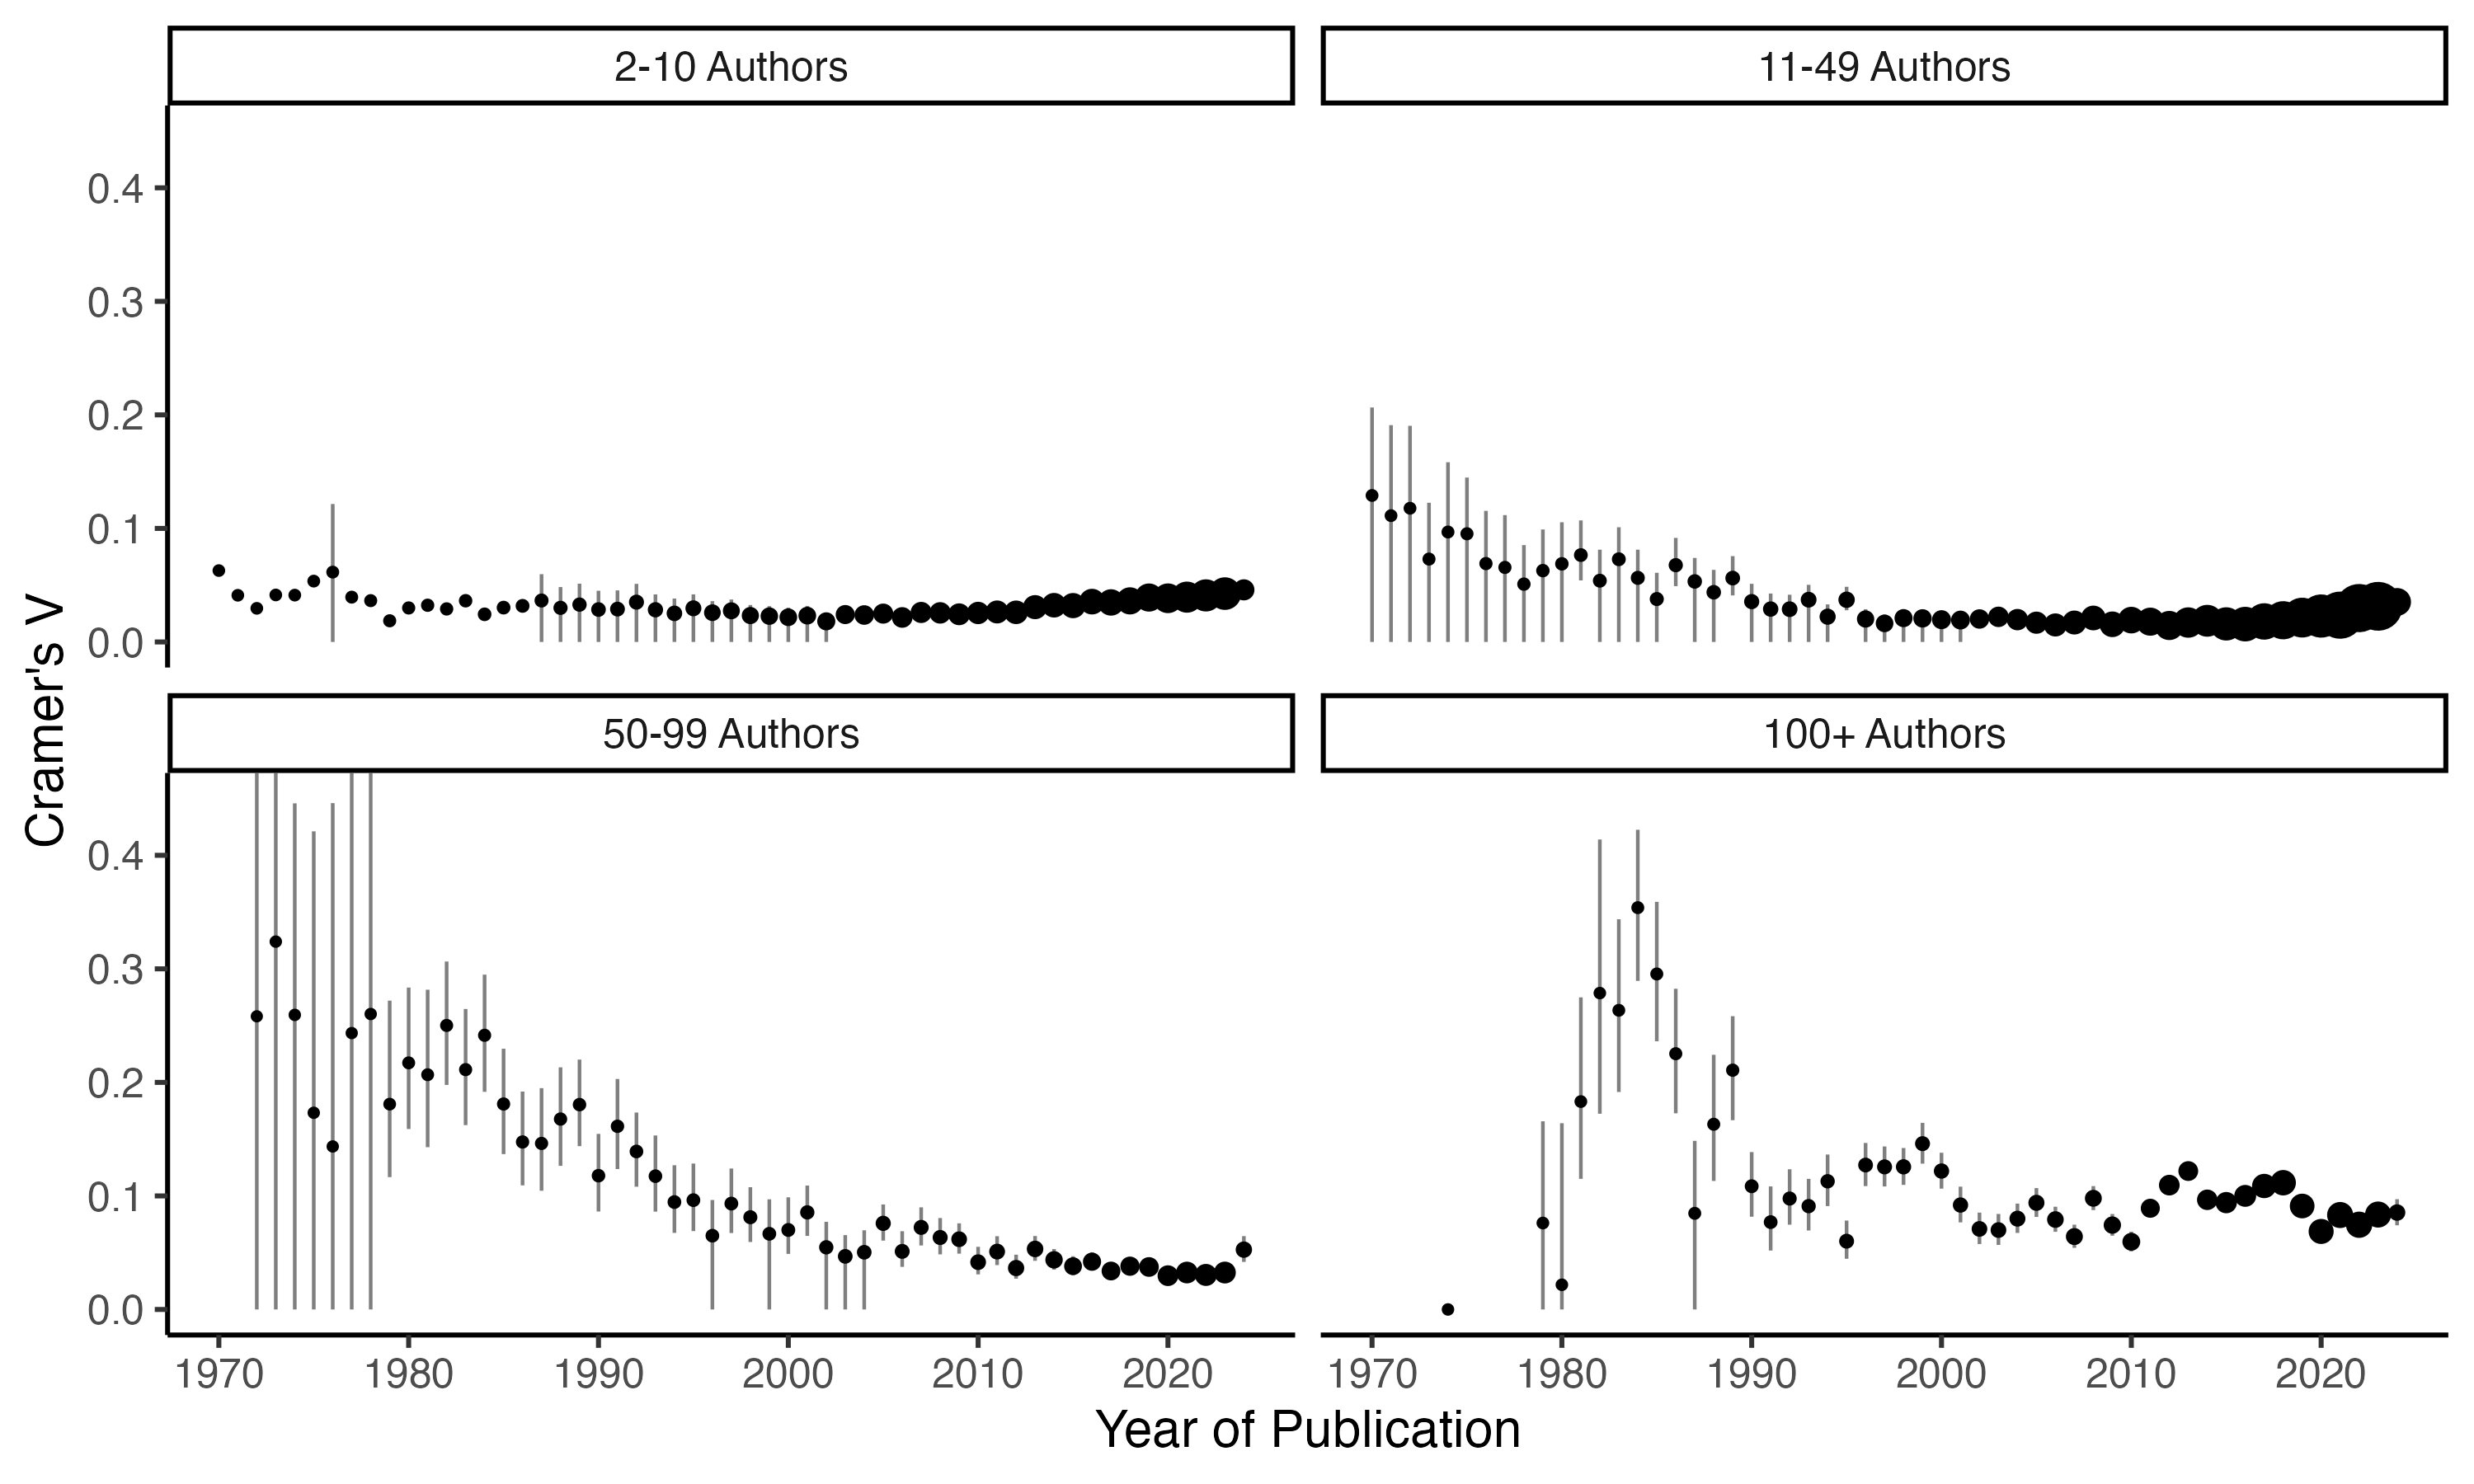
\includegraphics[width=1\linewidth]{figure/figure_8_author_effect_gpe} \caption{Effect size of the differences in representation for UN Regions for author affiliations in big-team science papers by year. Larger dots indicate more papers and authors represented in the calculation of effect size.}\label{fig:fig-effect-gpe}
\end{figure}

\begin{table}[tbp]

\begin{center}
\begin{threeparttable}

\caption{\label{tab:big-teams-table}Number of Authors and Papers by Subject Area}

\begin{tabular}{lccccc}
\toprule
Number of Authors & \multicolumn{1}{c}{Statistic} & \multicolumn{1}{c}{Health Sciences} & \multicolumn{1}{c}{Physical Sciences} & \multicolumn{1}{c}{Social Sciences} & \multicolumn{1}{c}{Life Sciences}\\
\midrule
2+ & Authors & 12,096,908 & 15,366,570 & 5,182,626 & 11,557,780\\
11+ & Authors & 2,726,450 & 1,513,520 & 445,271 & 2,208,278\\
50+ & Authors & 767,322 & 319,453 & 65,409 & 378,522\\
100+ & Authors & 502,493 & 217,863 & 34,708 & 214,346\\
2+ & Papers & 8,758,846 & 17,195,880 & 3,441,064 & 8,705,266\\
11+ & Papers & 507,871 & 255,587 & 38,011 & 352,012\\
50+ & Papers & 17,184 & 26,010 & 894 & 8,690\\
100+ & Papers & 5,429 & 15,009 & 242 & 2,622\\
\bottomrule
\addlinespace
\end{tabular}

\begin{tablenotes}[para]
\normalsize{\textit{Note.} Papers can be classified into multiple categories.}
\end{tablenotes}

\end{threeparttable}
\end{center}

\end{table}


\end{document}
